\subsection{仿射空间 E 的乘积分解}

我们沿用命题 5 的记号。对于 \(0 \leqslant p \leqslant s\) ，设 \(\mathbf{E}_p\) 为群 \(\mathbf{T}_p'\) 在 \(\mathbf{E}\) 中诸轨道所成的集合，\(\varphi_p\) 为从 \(\mathbf{E}\) 到 \(\mathbf{E}_p\) 的典范映射。\(\mathbf{T}\) 在 \(\mathbf{E}\) 上的作用可过渡到商；特别地，\(\mathbf{T}_p\) 作用于 \(\mathbf{E}_p\) ，并且立即可见（例如在 \(\mathbf{E}\) 中取一个原点），\(\mathbf{E}_p\) 是一个仿射空间，以 \(\mathbf{T}_p\) 为其平移空间。置 \(\mathbf{E}' = \mathbf{E}_0 \times \cdots \times \mathbf{E}_s\) ；这是一个仿射空间，以 \(\mathbf{T} = \mathbf{T}_0 \oplus \cdots \oplus \mathbf{T}_s\) 为其平移空间。设 \(\varphi : \mathbf{E} \to \mathbf{E}'\) 为诸 \(\varphi_p\) 的乘积映射；由于 \(\varphi\) 与 \(\mathbf{T}\) 的作用交换，它是一个双射，甚至是仿射空间的同构。在下文中，我们把 \(\mathbf{E}\) 与 \(\mathbf{E}'\) 依照 \(\varphi\) 等同起来；映射 \(\varphi_p\) 于是等同于 \(\mathbf{E}'\) 到 \(\mathbf{E}_p\) 上的典范投影。

由于 W 保持 \(T_{p}^{\prime}\) 稳定，W 在 E 上的作用过渡到商，并定义 W 在 \(E_{p}\) 上的一个作用（对于 \(0 \leqslant p \leqslant s\) ），从而由限制得到 \(W_{p}\) 在 \(E_{p}\) 上的一个作用（对于 \(1 \leqslant p \leqslant s\) ）。另一方面，设 C 是一个室，\(i \in I\) ，并设 p 是使 \(i \in J_{p}\) 的整数。对于任意 \(x \in E\) ，我们有

\[
s _ {i} (\mathrm{C}) (x) = x - \lambda . e _ {i} (\mathrm{C}) \quad \text { with } \quad \lambda \in \mathbf {R}.
\]

由于 \(e_i \in \mathbf{T}_q'\) （对于 \(q \neq p\) ），由此得到

\[
\varphi_ {q} (w (x)) = \varphi_ {q} (x) \text {for} x \in \mathrm{E}, w \in \mathrm{W} _ {p}; 0 \leqslant q \leqslant s \text {and} q \neq p.
\]

因此，若 \(w = w_{1} \ldots w_{s} \in \mathrm{W}\) ，其中 \(w_{p} \in \mathrm{W}_{p}\) （对于 \(1 \leqslant p \leqslant s\) ），则

\[
w \left(\left(x _ {0}, \dots , x _ {s}\right)\right) = \left(x _ {0}, w _ {1} \left(x _ {1}\right), \dots , w _ {s} \left(x _ {s}\right)\right)\tag{5}
\]

对所有 \(x_{p} \in E_{p}\) （对于 \(0 \leqslant p \leqslant s\) ）成立。换言之，W 在 \(E = E'\) 上的作用恰是诸 \(W_{p}\) 在 \(E_{p}\) 上作用的乘积（我们置 \(W_{0} = \{1\}\) ）。由此可知，\(W_{p}\) 忠实地作用于 \(E_{p}\) ，并且 \(W_{p}\) 可等同于欧氏空间 \(E_{p}\) 的一个位移群（当然，平移空间 \(T_{p}\) —— 即 \(E_{p}\) 的平移空间 —— 赋予由 T 上的标量积所诱导的标量积）。

命题 6. (i) 群 \(W_{p}\) 是欧氏仿射空间 \(E_{p}\) 的一个位移群；它由反射生成；赋予离散拓扑后，它适当地作用于 \(E_{p}\) ；它是不可约的。

\begin{enumerate}
\def\labelenumi{(\roman{enumi})}
\setcounter{enumi}{1}
\tightlist
\item
  设 \(\mathfrak{H}_p\) 为超平面 \(\mathrm{H}\)（在 \(\mathrm{E}_p\) 中且满足 \(s_{\mathrm{H}} \in \mathrm{W}_p\) ）所成的集合。集合 \(\mathfrak{H}\) 由形如
\end{enumerate}

\[
\mathrm{H} = \mathrm{E} _ {0} \times \mathrm{E} _ {1} \times \dots \times \mathrm{E} _ {p - 1} \times \mathrm{H} _ {p} \times \mathrm{E} _ {p + 1} \times \dots \times \mathrm{E} _ {s},
\]

其中 \(p = 1,\dots ,s\) 且 \(\mathrm{H}_p\in \mathfrak{H}_p\)

\begin{enumerate}
\def\labelenumi{(\roman{enumi})}
\setcounter{enumi}{2}
\tightlist
\item
  每个室 C 都形如 \(E_{0} \times C_{1} \times \cdots \times C_{s}\) ，其中对每个 p，集合 \(C_{p}\) 都是 \(E_{p}\) 中由超平面集 \(H_{p}\) 所定义的一个室；此外，\(C_{p}\) 的墙是超平面 \(\varphi_{p}(H_{i}(C))\) ，其中 \(i \in J_{p}\) 。
\end{enumerate}

设 \(\mathbf{C}\) 是一个室。置 \(\mathrm{H}_i = \mathrm{H}_i(\mathrm{C})\) ，\(e_i = e_i(\mathrm{C})\) 且 \(s_i = s_i(\mathrm{C})\) （对于 \(i \in \mathbb{I}\) ，沿用第 4 号的记号）。

\begin{enumerate}
\def\labelenumi{(\roman{enumi})}
\tightlist
\item
  设 \(i\) 属于 \(\mathbf{J}_p\) ；由于 \(e_i \in \mathrm{T}_p\) 且 \(\mathrm{T}\) 是两两正交的子空间 \(\mathrm{T}_0, \mathrm{T}_1, \ldots, \mathrm{T}_s\) 的直和，\(\mathrm{T}\) 中与 \(e_i\) 正交的超平面形如 \(\mathrm{L}_i + \mathrm{T}_p'\) ，其中 \(\mathrm{L}_i\) 是 \(\mathrm{T}_p\) 中与 \(e_i\) 正交的超平面。仿射超平面 \(\mathrm{H}_i\) （\(\mathrm{E}\) 中的）形如 \(\mathrm{L}_i + \mathrm{T}_p' + x\) ，其中 \(x \in \mathrm{E}\) ，并且我们有
\end{enumerate}

\[
\mathrm{H} _ {i} = \mathrm{E} _ {0} \times \mathrm{E} _ {1} \times \dots \times \mathrm{E} _ {p - 1} \times \mathrm{H} _ {i} ^ {\prime} \times \mathrm{E} _ {p + 1} \times \dots \times \mathrm{E} _ {s}\tag{6}
\]

其中 \(H_{i}^{\prime}=L_{i}+\varphi_{p}(x)=\varphi_{p}(H_{i})\) 。现在立即可见，\(s_{i}\) 在 \(E_{p}\) 上的作用是超平面 \(H_{i}^{\prime}\) （\(E_{p}\) 中的）所对应的反射。于是，群 \(W_{p}\) 是 \(E_{p}\) 中由反射生成的位移群；适当性判别准则 (D'2) 的验证是直接的。最后，命题 5 (v) 表明 \(W_{p}\) 不可约。这就证明了 (i)。

\begin{enumerate}
\def\labelenumi{(\roman{enumi})}
\setcounter{enumi}{1}
\tightlist
\item
  由定理 1 的推论，集合 \(\mathfrak{H}_p\) 由形如 \(w_p(\mathrm{H}_i')\) 的超平面组成，其中 \(i\) 属于 \(\mathrm{J}_p\) 且 \(w_p\) 属于 \(\mathrm{W}_p\) 。进而，若 \(w = w_1 \ldots w_s\) 且 \(w_p \in \mathrm{W}_p\) （对所有 \(p\) ），则公式 (5) 与 (6) 蕴含
\end{enumerate}

\[
w (\mathrm{H} _ {i}) = \mathrm{E} _ {0} \times \mathrm{E} _ {1} \times \dots \times \mathrm{E} _ {p - 1} \times w _ {p} (\mathrm{H} _ {i} ^ {\prime}) \times \mathrm{E} _ {p + 1} \times \dots \times \mathrm{E} _ {s},\tag{7}
\]

由此立得 (ii)。

\begin{enumerate}
\def\labelenumi{(\roman{enumi})}
\setcounter{enumi}{2}
\tightlist
\item
  设 \(i\) 属于 \(\mathbf{J}_p\) ；由公式 (6)，开半空间 \(D_i\) （由 \(\mathbf{H}_i\) 界定且包含 \(C\) ）形如
\end{enumerate}

\[
\mathrm{D} _ {i} = \mathrm{E} _ {0} \times \mathrm{E} _ {1} \times \dots \times \mathrm{E} _ {p - 1} \times \mathrm{D} _ {i} ^ {\prime} \times \mathrm{E} _ {p + 1} \times \dots \times \mathrm{E} _ {s},
\]

其中 \(D_{i}^{\prime}\) 是一个由 \(H_{i}^{\prime}\) 界定的开半空间（在 \(E_{p}\) 中）。置 \(C_{p} = \bigcap_{i \in J_{p}} D_{i}^{\prime}\) ；由于 \(C = \bigcap_{i \in I} D_{i}\) ，立即可得

\[
\mathrm{C} = \mathrm{E} _ {0} \times \mathrm{C} _ {1} \times \dots \times \mathrm{C} _ {s};
\]

因此，诸集合 \(C_{p}\) 都非空，且由于 C 不与属于 H 的任何超平面相交，集合 \(C_{p}\) 不与属于 \(H_{p}\) 的任何超平面相交。于是 §1 第 3 号命题 5 表明，\(C_{p}\) 是由 \(H_{p}\) 在 \(E_{p}\) 中定义的一个室。利用 §1 第 2 号命题 4，容易看出 \(C_{p}\) 的墙是超平面 \(H_{i}^{\prime} = \varphi_{p}(H_{i})\) ，其中 \(i \in J_{p}\) 。

\subsection{室的结构}

设 \(\mathbf{C}\) 是一个室，\(\mathfrak{M}\) 是 \(\mathbf{C}\) 的墙集，并且对于 \(\mathrm{H} \in \mathfrak{M}\) ，设 \(e_{\mathrm{H}}\) 为与 \(\mathrm{H}\) 正交、关于 \(\mathrm{H}\) 与 \(\mathbf{C}\) 位于同侧的单位向量。

命题 7. 假设群 W 是本质的且是有限的。则：

\begin{enumerate}
\def\labelenumi{(\roman{enumi})}
\item
  存在唯一的点 \(a\) 属于 \(\mathbf{E}\) 且在 \(\mathbf{W}\) 下不变。
\item
  族 \((e_{\mathsf{H}})_{\mathsf{H}\in \mathfrak{M}}\) 是 \(\mathrm{T}\) 的一组基。
\item
  室 C 是以 a 为顶点、由 T 的基 \((e_{\mathrm{H}}^{\prime})_{\mathrm{H}\in \mathfrak{M}}\) （它满足 \((e_{\mathrm{H}}|e_{\mathrm{H}'}') = \delta_{\mathrm{HH}'}\) ）所确定的开单形锥。
\item
  由第 6 号命题 4，存在一点 \(a \in E\) 在 W 下不变。设 \(t \in T\) 使得 \(t + a\) 在 W 下不变。对所有 \(w \in W\) ，
\end{enumerate}

\[
\mathrm{U} (w). t + a = w (t + a) = t + a,
\]

于是 \(\mathrm{U}(w).t = t\) ；由于 \(\mathrm{W}\) 是本质的，这蕴含 \(t = 0\) ，从而证明了 \(a\) 的唯一性。

\begin{enumerate}
\def\labelenumi{(\roman{enumi})}
\setcounter{enumi}{1}
\item
  由于 W 是本质的，按第 7 号的记号有 \(T = T_{1}\) ，且命题 5 (iv) 表明族 \((e_{\mathrm{H}})_{\mathrm{H}\in\mathfrak{M}}\) 生成向量空间 T。E 中存在在 W 下不变的点这一事实表明族 \((e_{\mathrm{H}})_{\mathrm{H}\in\mathfrak{M}}\) 是自由的（第 6 号，命题 4）。
\item
  设 \(a\) 是 \(\mathbf{E}\) 的在 \(\mathbf{W}\) 下不变的唯一点。由于 \((e_{\mathrm{H}})_{\mathrm{H}\in \mathfrak{M}}\) 是 \(\mathbf{T}\) 的一组基，且标量积是 \(\mathbf{T}\) 上的非退化双线性型，故存在唯一的基 \((e_{\mathrm{H}}^{\prime})_{\mathrm{H}\in \mathfrak{M}}\) （属于 \(\mathbf{T}\) ），使得 \((e_{\mathrm{H}}|e_{\mathrm{H}'}') = \delta_{HH'}\) 对 \(\mathrm{H},\mathrm{H}'\) 属于 \(\mathfrak{M}\) 成立。每一点 \(x\) （\(\mathbf{E}\) 中的）都可唯一地写成形式 \(x = t + a\) ，其中 \(t = \sum_{\mathrm{H}\in \mathfrak{M}}\xi_{\mathrm{H}}.e_{\mathrm{H}}'\) 且诸 \(\xi_{\mathrm{H}}\) 为实数。于是 \(x\) 属于 \(\mathbf{C}\) 当且仅当：对每个超平面 \(\mathrm{H}\in \mathfrak{M}\) ，\(x\) 位于 \(\mathbf{H}\) 的与 \(e_{\mathrm{H}}\) 相同的一侧，换言之 \((t|e_{\mathrm{H}}) = \xi_{\mathrm{H}}\) 严格为正。由此得 (iii)。
\end{enumerate}

命题 8. 假设群 W 是本质的、不可约的且无限的。则：

\begin{enumerate}
\def\labelenumi{(\roman{enumi})}
\item
  E 中没有在 W 下不变的点。
\item
  我们有 \(\operatorname{Card} \mathfrak{M} = \dim T + 1\) ，并且存在实数 \(c_{\mathrm{H}} > 0\) 使得 \(\sum_{\mathrm{H} \in \mathfrak{M}} c_{\mathrm{H}} \cdot e_{\mathrm{H}} = 0\) 。若实数 \(c_{\mathrm{H}}'\) 满足 \(\sum_{\mathrm{H} \in \mathfrak{M}} c_{\mathrm{H}}' \cdot e_{\mathrm{H}} = 0\) ，则存在实数 \(\xi\) 使得 \(c_{\mathrm{H}}' = \xi c_{\mathrm{H}}\) 对 \(\mathfrak{M}\) 中所有 H 成立。
\item
  室 C 是一个开单形。
\end{enumerate}

断言 (i) 由命题 4 得出。另一方面，由于 W 是本质的，向量 \((e_{\mathrm{H}})_{\mathrm{H}\in\mathfrak{M}}\) 生成 T。我们有 \((e_{\mathrm{H}}|e_{\mathrm{H}^{\prime}})\leqslant0\) （对于 \(H,H^{\prime}\in \mathfrak{M}\) 且 \(H\neq H^{\prime}\) ；命题 3），并且由于 W 不可约，不存在把 \(\mathfrak{M}\) 分成两个不相交子集 \(\mathfrak{M}^{\prime}\) 与 \(\mathfrak{M}^{\prime\prime}\) 的分割，使得 \(H^{\prime}\in \mathfrak{M}^{\prime}\) 与 \(H^{\prime\prime}\in \mathfrak{M}^{\prime\prime}\) 蕴含 \((e_{\mathrm{H}^{\prime}}|e_{\mathrm{H}^{\prime\prime}})=0\) 。于是可以应用第 5 号引理 5，且该引理的情形 1) 被排除；事实上，诸 \(e_{H}\) 不是线性无关的，因为 W 没有不动点。断言 (ii) 由此得证。

现在证明 (iii)。把 C 的墙编号为 \(H_{0}, H_{1}, \ldots, H_{d}\) ，并置 \(t_{m} = e_{H_{m}}\) 。由 (ii)，向量 \(t_{1}, \ldots, t_{d}\) 构成 T 的一组基，因此超平面 \(H_{1}, \ldots, H_{d}\) 有一个公共点 \(a_{0}\) ，并且存在 T 的一组基 \((t_{1}^{\prime}, \ldots, t_{d}^{\prime})\) 使得 \((t_{m}|t_{n}^{\prime}) = \delta_{mn}\) ；此外，仍由 (ii)，存在实数 \(c_{1} > 0, \ldots, c_{d} > 0\) 使得

\[
t _ {0} = - \left(c _ {1}. t _ {1} + \dots + c _ {d}. t _ {d}\right).
\]

由于向量 \(t_{0}\) 与超平面 \(H_{0}\) 正交，存在实数 c 使得 \(H_{0}\) 是 E 中形如 \(x = t + a_{0}\) 且满足 \((t|t_{0}) = -c\) 的点所成的集合。

E 的每一点都可唯一地写成形式 \(x = t + a_{0}\) ，其中 \(t = \xi_{1}.t_{1}^{\prime} + \cdots + \xi_{d}.t_{d}^{\prime}\) 且 \(\xi_{1}, \ldots, \xi_{d}\) 为实数。点 x 属于 C 当且仅当它位于 \(H_{m}\) 的与 \(t_{m}\) 相同的一侧（对于 \(0 \leqslant m \leqslant d\) ）；这可翻译为不等式 \((t|t_{1}) > 0, \ldots, (t|t_{d}) > 0\) 与 \((t|t_{0}) > -c\) ，或等价地 \(\xi_{1} > 0, \ldots, \xi_{d} > 0\) ，\(c_{1}\xi_{1} + \cdots + c_{d}\xi_{d} < c\) 。由于 C 非空，故 c \textgreater{} 0。置 \(a_{m} = a_{0} + \frac{c}{c_{m}}.t_{m}'\) （对于 \(1 \leqslant m \leqslant d\) ）；于是室 C 由 E 中形如 \(a_{0} + \sum_{m=1}^{d} \lambda_{m}.(a_{m} - a_{0})\) 且满足 \(\lambda_{1} > 0, \ldots, \lambda_{d} > 0\) 与 \(\lambda_{1} + \cdots + \lambda_{d} < 1\) 的点组成，故 C 是以 \(a_{0}, \ldots, a_{d}\) 为顶点的开单形。证毕。

注. 1) 如第 8 号中那样，把 E 与 \(E_{0} \times E_{1} \times \cdots \times E_{s}\) 等同，把 W 与 \(W_{1} \times \cdots \times W_{s}\) 等同。由命题 6，室 C 于是等同于

\[
\mathrm{E} _ {0} \times \mathrm{C} _ {1} \times \dots \times \mathrm{C} _ {s},
\]

其中 \(C_{p}\) 是 \(E_{p}\) 中相对于超平面集 \(H_{p}\) 的一个室。由命题 7 与 8，诸室 \(C_{1},\ldots,C_{s}\) 中的每一个都是开单形锥或开单形。

\begin{enumerate}
\def\labelenumi{\arabic{enumi})}
\setcounter{enumi}{1}
\tightlist
\item
  假设 W 不可约且本质。若 H 与 \(H'\) 是 C 的两面墙，则 \(m_{HH'} = +\infty\) 当且仅当 \(e_{H} = -e_{H'}\) （命题 3）。由命题 7 与 8，这只可能发生在 H 与 \(H'\) 是 C 仅有的墙且 E 的维数为 1 的情形。于是，诸 \(m_{HH'}\) 中之一为无穷的唯一情形是：E 的维数为 1 且群 W 由两个不同点所关联的反射生成（参见~§2，第 4 号）。
\end{enumerate}

在一般情形，与 W 相关联的 Coxeter 矩阵的元素都是有限的，除非 \(E_{1},\ldots,E_{s}\) 中至少有一个属于前述类型。

\subsection{特殊点}

设 L 是属于 W 的平移所成的集合，并设 \(\Lambda\) 为由这样的 \(t \in T\) 组成的集合：平移 \(x \mapsto t + x\) 属于 L。立即可见 \(\Lambda\) 在 U(W) 下稳定，且 L 是 W 的正规子群。由于 W 适当地作用于 E，L 亦然，从而容易得出 \(\Lambda\) 是 T 的离散子群。对 E 的任意一点 x，记 \(W_x\) 为 x 在 W 中的稳定子。

命题 9. 设 \(a \in E\) 。下列条件等价：

\begin{enumerate}
\def\labelenumi{(\roman{enumi})}
\item
  我们有 \(\mathrm{W} = \mathrm{W}_{a}.\mathrm{L}\) ；
\item
  同态 U 在 \(W_{a}\) 上的限制是从 \(W_{a}\) 到 \(\mathrm{U}(\mathrm{W})\) 的同构；
\item
  对每个超平面 \(\mathbf{H} \in \mathfrak{H}\) ，存在超平面 \(\mathbf{H}' \in \mathfrak{H}\) 平行于 \(\mathbf{H}\) 且使得 \(a \in \mathbf{H}'\) 。
\end{enumerate}

显然 (i) \(\Leftrightarrow\) (ii)，因为 L 是 U 的核且 \(\mathrm{L} \cap \mathrm{W}_a = \{1\}\) 。

假设 (i)，并设 \(\mathbf{H} \in \mathfrak{H}\) ；则 \(s_{\mathbf{H}} \in \mathbf{W}_a\) . L，于是存在向量 \(t \in \Lambda\) 使得 \(a = s_{\mathbf{H}}(a) + t\) ；向量 \(t\) 与 \(\mathbf{H}\) 正交，且若 \(\mathrm{H}' = \mathrm{H} + \frac{1}{2} t\) ，则 \(s_{\mathbf{H}'}(x) = s_{\mathbf{H}}(x) + t\) （对所有 \(x \in \mathbf{E}\) ；参见~§2，第 4 号，命题 5）。由于 \(t \in \Lambda\) 且 \(s_{\mathbf{H}} \in \mathbf{W}\) ，我们有 \(s_{\mathbf{H}'} \in \mathbf{W}\) ，从而 \(\mathrm{H}' \in \mathfrak{H}\) ；我们还有 \(a = s_{\mathbf{H}'}(a)\) ，从而 \(a \in \mathbf{H}'\) 。于是 (i) 蕴含 (iii)。

假设 (iii)。设 \(\mathrm{H} \in \mathfrak{H}\) ；取 (iii) 中的 \(\mathrm{H}'\) 。则 \(s_{\mathrm{H}'}(a) = a\) ，故 \(s_{\mathrm{H}'} \in \mathrm{W}_a\) ；由于 \(\mathrm{H}\) 平行于 \(\mathrm{H}'\) ，元素 \(w = s_{\mathrm{H}'} s_{\mathrm{H}}\) （\(\mathrm{W}\) 中的）是一个平移（§2，第 4 号，命题 5），故 \(w \in \mathrm{L}\) ；于是 \(s_{\mathrm{H}} = s_{\mathrm{H}'} w \in \mathrm{W}_a\) . L。由于 \(\mathrm{W}\) 由族 \((s_{\mathrm{H}})_{\mathrm{H} \in \mathfrak{H}}\) 生成，可得 \(\mathrm{W} = \mathrm{W}_a\) . L，因而 (iii) 蕴含 (i)。

定义 1. 一点 \(a\) （属于 \(E\) ）若满足命题 9 中的等价条件，就称为 \(W\) 的特殊点。

显然 E 的特殊点所成的集合在 W 下稳定。

命题 10. 存在 W 的一个特殊点。

由第 8 号命题 6，只需考虑 W 是本质的情形。T 的自同构群 U(W) 是有限的（参见~第 6 号，定理 3），且对每个超平面 H，\(U(s_{H})\) 是一个正交反射；此外，U(W) 由族 \((U(s_{H}))_{H \in \mathfrak{H}}\) 生成。由第 9 号命题 7，存在 T 的一组基 \((e_{i})_{i \in I}\) ，使得群 U(W) 由按下式定义的反射集 \((s_{i})_{i \in I}\) 生成：

\[
s _ {i} (t) = t - 2 (t | e _ {i}). e _ {i}.
\]

第 2 号定理 1 的推论表明，每个反射 \(s \in \mathrm{U}(\mathrm{W})\) 都形如 \(s = \mathrm{U}(s_{\mathrm{H}})\) ，其中 \(\mathrm{H} \in \mathfrak{H}\) 。于是可以在 \(\mathfrak{H}\) 中找到一族超平面 \((\mathbf{H}_i)_{i \in I}\) ，使得 \(s_i = \mathrm{U}(s_{\mathrm{H}_i})\) 对所有 \(i\) 成立。由于诸向量 \(e_i\) 线性无关，存在 \(a \in E\) 使得 \(a \in H_i\) 对所有 \(i \in I\) 成立。我们有 \(s_{\mathrm{H}_i} \in W_a\) ，故 \(\mathrm{U}(\mathrm{W}) = \mathrm{U}(\mathrm{W}_a)\) ，这意味着 \(W = W_a.L\) ，因为 \(L\) 是 \(U\) 的核。于是 \(a\) 是特殊点。

当 W 有限且本质时，W 只有唯一的特殊点，即在 W 下不变的唯一点。因此，对特殊点的考察主要在 W 无限时才有意义。

命题 11. 假设 W 是本质的。设 a 是 W 的一个特殊点。相对于 \(W_{a}\) 的诸室是以 a 为顶点的开单形锥。对每个室 \(C'\) （相对于 \(W_{a}\) ），存在唯一一个相对于 W 的室 C，它包含于 \(C'\) 且满足 \(a \in \overline{C}\) 。诸 \(w'(\overline{C})\) （\(w' \in W_{a}\) ）的并是 a 在 E 中的一个闭邻域。\(C'\) 的每面墙都是 C 的墙。若 W 无限且不可约，则 C 的墙是 \(C'\) 的墙加上一个不与 \(C'\) 的墙平行的仿射超平面。

设 \(\mathfrak{H}'\) 为满足 \(H \in \mathfrak{H}\) 且包含 \(a\) 的 H 所成的集合。群 \(W_a\) 由诸 \(s_H\) （\(H \in \mathfrak{H}'\) ）生成（第 3 号，命题 2）。相对于 \(W_a\) 的诸室是以 \(a\) 为顶点的开单形锥（第 9 号，命题 7）。设 \(C'\) 是这样一个室，\(U\) 是以 \(a\) 为中心、不与 \(\mathfrak{H} - \mathfrak{H}'\) 中任何元素相交的非空开球。由于 \(a \in \overline{C'}\) ，存在一点 \(b\) 属于 \(U \cap C'\) 。于是 \(b \notin H\) 对所有 \(H \in \mathfrak{H}\) 成立，从而 \(b\) 属于一个室 \(C\) （相对于 \(\mathfrak{H}\) ）。由于 \(\mathfrak{H}' \subset \mathfrak{H}\) ，我们有 \(C \subset C'\) 。集合 \(U \cap C'\) 不与任何 \(H \in \mathfrak{H}\) 相交且是凸的，故 \(U \cap C' \subset C\) ；于是 \(a \in \overline{C}\) 。反之，设 \(C_1\) 是相对于 \(W\) 、包含于 \(C'\) 且满足 \(a \in \overline{C}_{1}\) 的一个室；则 \(C_{1}\) 与 U 相交，且 \(U \cap C_{1} \subset U \cap C' = U \cap C\) ；室 C 与 \(C_{1}\) 有公共点，故必重合。对任意 \(w' \in W_{a}\) ，我们有 \(w'(U) = U\) ，于是

\[
\mathrm{U} \cap w ^ {\prime} (\mathrm{C}) = w ^ {\prime} (\mathrm{U} \cap \mathrm{C}) = w ^ {\prime} (\mathrm{U} \cap \mathrm{C} ^ {\prime}) = \mathrm{U} \cap w ^ {\prime} (\mathrm{C} ^ {\prime});
\]

由于诸 \(w'(C)\) （\(w' \in W_a\) ）的并在 \(E\) 中稠密，诸 \(U \cap w'(C) = U \cap w'(C')\) 的并在 \(U\) 中稠密，从而诸 \(w'(\overline{C})\) （\(w' \in W_a\) ）的并包含 \(U\) 。最后，若 \(H\) 是 \(C'\) 的一面墙，则存在一点 \(c \in U \cap H\) 以及开邻域 \(V \subset U\) （\(c\) 的），使得 \(V \cap C'\) 是 \(V\) 与由 \(H\) 界定且包含 \(C'\) 的开半空间之交；由于 \(V \cap C' = V \cap U \cap C' = V \cap U \cap C = V \cap C\) ，可知 \(H\) 是 \(C\) 的一面墙。若 \(W\) 无限且不可约，则 \(C\) 是一个开单形（第 9 号，命题 8），因而比开单形锥 \(C'\) 多一面墙。

推论. 假设 W 是本质的。

\begin{enumerate}
\def\labelenumi{(\roman{enumi})}
\item
  若 \(a \in \mathbb{E}\) 是特殊的，则存在一个室 \(\mathbb{C}\) 使得 \(a\) 是 \(\overline{\mathbb{C}}\) 的一个极点。
\item
  若 \(\mathrm{C}\) 是一个室，则存在 \(\overline{\mathrm{C}}\) 的一个极点，它是特殊点。
\end{enumerate}

第一个断言由命题 11 得出。第二个断言由第一个以及 W 传递地作用于室集这一事实得出。

然而，\(\overline{C}\) 的极点未必是 W 的特殊点（参见~第 VI 章，图版 X，\(B_{2}\) 型与 \(G_{2}\) 型）。

注. 1) 假设 W 本质、不可约且无限，并沿用命题 11 的记号。由于 U 是从 \(W_{a}\) 到 \(U(W)\) 的同构，可知位移群 \(U(W)\) （它由诸反射 \(U(s_{H})\) （\(H \in \mathfrak{H}\) ）生成）的 Coxeter 图，可由 W 的 Coxeter 图删去顶点 i（它对应于 C 的唯一一面不是 \(C'\) 的墙）而得到。

命题 12. 假设 W 是本质的。设 a 是一个特殊点，L(a) 是 a 在平移群 L 下的诸像所成的集合，并设 C 是一个室。则 \(\overline{C}\) 与 L(a) 交于唯一点；该点是 \(\overline{C}\) 的一个极点。

存在一个室 \(C_{1}\) 使得 a 是 \(\overline{C}_{1}\) 的极点（命题 11 的推论）。每个室都形如 \(\mathbf{C}=tw^{\prime}(\mathbf{C}_{1})\) ，其中 \(w^{\prime}\in W_{a}\) 且 \(t\in L\) ，因为 \(W=W_{a}.L\) ；于是 \(tw^{\prime}(a)=t(a)\in\mathrm{L}(a)\) 是 \(\overline{C}\) 的一个极点。另一方面，\(\overline{C}\) 不可能包含 \(\mathrm{L}(a)\) 中两个不同的点，因为 \(\overline{C}\) 是 W 的基本域（第 3 号，定理 2）。

注. 2) 集合 L(a) 包含于特殊点集，但一般与它不同（参见~第 VI 章，§2，第 2 号以及图版 I 至 VI）。

\section{Coxeter 群的几何表示}

在本段中，所考虑的向量空间都是实向量空间。

\subsection{与 Coxeter 群相关联的型}

设 \(S\) 是一个集合，\(M = (m(s, s')_{s, s' \in S})\) 是 \(S\) 型的一个 Coxeter 矩阵（第 IV 章，§1，第 9 号）。回忆一下，这意味着：

\begin{enumerate}
\def\labelenumi{(\arabic{enumi})}
\item
  \(M\) 的元素是整数或 \(+\infty\) 。
\item
  M 是对称的。
\item
  \(m(s, s) = 1\) 对所有 s 成立。
\item
  \(m(s, s') \geqslant 2\) （对于 \(s \neq s'\) ）。
\end{enumerate}

设 \(\mathbf{E} = \mathbf{R}^{(\mathrm{S})}\) ，\((e_s)_{s \in S}\) 是 \(\mathbf{E}\) 的典范基，\(B_M\) 是 \(\mathbf{E}\) 上满足下式的双线性型：

\[
\mathrm{B} _ {\mathrm{M}} (e _ {s}, e _ {s ^ {\prime}}) = - \cos \frac {\pi}{m (s , s ^ {\prime})}.
\]

型 \(B_{M}\) 是对称的。它称为矩阵 M 的关联型。我们有

\[
\mathrm{B} _ {\mathrm{M}} \left(e _ {s}, e _ {s}\right) = 1 \text {and} \mathrm{B} _ {\mathrm{M}} \left(e _ {s}, e _ {s ^ {\prime}}\right) \leqslant 0 \text {if} s \neq s ^ {\prime}.
\]

设 \(s \in S\) ，\(f_s\) 是线性型 \(x \mapsto 2B_M(e_s, x)\) 。我们用 \(\sigma_s\) 表示由对 \((e_s, f_s)\) 定义的伪反射（参见~§2，第 1 号）；由于 \(\langle e_s, f_s \rangle = 2\) ，它是一个反射（§2，第 2 号）。我们有

\[
\sigma_ {s} (x) = x - 2 \mathrm{B} _ {\mathrm{M}} (e _ {s}, x). e _ {s}
\]

并且特别地

\[
\sigma_ {s} (e _ {s ^ {\prime}}) = e _ {s ^ {\prime}} + 2 \cos \frac {\pi}{m (s , s ^ {\prime})}. e _ {s}.
\]

由于 \(e_{s}\) 关于 \(B_{M}\) 不是迷向的，空间 E 是直线 \(Re_{s}\) 与超平面 \(H_{s}\) （正交于 \(e_{s}\) ）的直和。由于 \(\sigma_{s}\) 在 \(Re_{s}\) 上等于 -1 且在 \(H_{s}\) 上等于 1，可知 \(\sigma_{s}\) 保持型 \(B_{M}\) 。当 S 有限且 \(B_{M}\) 非退化时（这种情形我们将在第 8 号中回到），可知 \(\sigma_{s}\) 是一个正交反射（ \(\S2\) ，第 3 号）。

\subsection{\texorpdfstring{平面 \(E_{s,s'}\) 与由 \(\sigma_{s}\) 和 \(\sigma_{s'}\) 生成的群}{平面 E\_s,s' 与由 sigma\_s 和 sigma\_s' 生成的群}}

在本号中，我们用 \(s\) 与 \(s'\) 表示 \(S\) 的两个满足 \(s \neq s'\) 的元素。置 \(m = m(s, s')\) ，并用 \(\mathrm{E}_{s,s'}\) 表示平面 \(\mathbf{Re}_s \oplus \mathbf{Re}_{s'}\) 。

命题 1. \(B_{M}\) 在 \(E_{s,s'}\) 上的限制是正的，且它非退化当且仅当 \(m\) 有限。

设 \(z = xe_{s} + ye_{s'}\) （其中 \(x, y \in \mathbf{R}\) ）是 \(E_{s,s'}\) 的一个元素。我们有

\[
\begin{array}{r} B _ {M} (z, z) = x ^ {2} - 2 x y \cos \frac {\pi}{m} + y ^ {2} \\ = (x - y. \cos \frac {\pi}{m}) ^ {2} + y ^ {2} \sin^ {2} \frac {\pi}{m}, \end{array}
\]

这表明 \(\mathrm{B}_{\mathsf{M}}\) 在 \(\mathrm{E}_{s,s'}\) 上是正的，并且它在该处非退化当且仅当 \(\sin \frac{\pi}{m} \neq 0\) 。命题得证。

反射 \(\sigma_{s}\) 与 \(\sigma_{s'}\) 保持 \(E_{s,s'}\) 稳定。我们将确定 \(\sigma_{s}\sigma_{s'}\) 在 \(E_{s,s'}\) 上限制的阶。我们区分两种情形：

\begin{enumerate}
\def\labelenumi{\alph{enumi})}
\tightlist
\item
  \(m = +\infty\)
\end{enumerate}

设 \(u = e_s + e_{s'}\) 。我们有 \(\mathrm{B}_{\mathrm{M}}(u, e_s) = \mathrm{B}_{\mathrm{M}}(u, e_{s'}) = 0\) ，故 \(u\) 在 \(\sigma_s\) 与 \(\sigma_{s'}\) 下不变。此外，

\[
\sigma_ {s} \left(\sigma_ {s ^ {\prime}} \left(e _ {s}\right)\right) = \sigma_ {s} \left(e _ {s} + 2 e _ {s ^ {\prime}}\right) = 3 e _ {s} + 2 e _ {s ^ {\prime}} = 2 u + e _ {s},
\]

从而

\[
\left(\sigma_ {s} \sigma_ {s ^ {\prime}}\right) ^ {n} \left(e _ {s}\right) = 2 n u + e _ {s} \text {   for   all   } n \in \mathbf {Z}.
\]

由此可知，\(\sigma_s\sigma_{s'}\) 在 \(\mathrm{E}_{s,s'}\) 上的限制是无限阶的。

\begin{enumerate}
\def\labelenumi{\alph{enumi})}
\setcounter{enumi}{1}
\tightlist
\item
  \(m\) 是有限的。
\end{enumerate}

型 \(B_{M}\) 给 \(E_{s,s'}\) 赋予欧氏平面的结构。由于 \(e_{s}\) 与 \(e_{s'}\) 的标量积等于 \(-\cos\frac{\pi}{m}=\cos\left(\pi-\frac{\pi}{m}\right)\) ，我们可以给 \(E_{s,s'}\) 定向，使得半直线 \(R_{+}e_{s}\) 与 \(R_{+}e_{s'}\) 之间的角等于 \(\pi-\frac{\pi}{m}\) 。若 D 与 \(D'\) 表示正交于 \(e_{s}\) 与 \(e_{s'}\) 的直线，

\[
(\widehat {D ^ {\prime} , D}) = \pi - (\widehat {D , D ^ {\prime}}) = \frac {\pi}{m}.
\]

现在，限制 \(\overline{\sigma}_s\) 与 \(\overline{\sigma}_{s'}\) （即 \(\sigma_s\) 与 \(\sigma_{s'}\) 在 \(E_{s,s'}\) 上的限制）是关于 D 与 \(D'\) 的正交对称。由 §2 第 5 号命题 6 的推论，可知 \(\overline{\sigma}_s\overline{\sigma}_{s'}\) 是角为 \(\frac{2\pi}{m}\) 的旋转。特别地，它的阶是 \(m\) 。

现在回到 E：

命题 2. \(\mathbf{GL}(\mathrm{E})\) 中由 \(\sigma_s\) 与 \(\sigma_{s'}\) 生成的子群是 \(2m(s,s')\) 阶的二面体群。

由于 \(\sigma_s\) 与 \(\sigma_{s'}\) 都是 2 阶的且互不相同，只需证明它们的乘积 \(\sigma_s\sigma_{s'}\) 的阶是 \(m(s,s')\) 。当 \(m(s,s')\) 无限时，这由上面的 a) 得出。当 \(m(s, s')\) 有限时，由命题 1 可知 E 是 \(E_{s,s'}\) 与其正交补 \(V_{s,s'}\) 的直和；由于 \(\sigma_s\) 与 \(\sigma_{s'}\) 在 \(V_{s,s'}\) 上是恒等，且由 b) 知 \(\sigma_s\sigma_{s'}\) 在 \(E_{s,s'}\) 上的限制的阶是 \(m(s, s')\) ，故 \(\sigma_s\sigma_{s'}\) 的阶确实等于 \(m(s, s')\) 。

\subsection{与 Coxeter 矩阵相关联的群和表示}

我们沿用前面各号的记号。设 \(W = W(M)\) 为由生成元族 \((g_{s})_{s \in S}\) 以及关系式 \(^{1}\)

\[
\left(g _ {s} g _ {s ^ {\prime}}\right) ^ {m \left(s, s ^ {\prime}\right)} = 1, \quad \text { for } s, s ^ {\prime} \in S, m \left(s, s ^ {\prime}\right) \neq + \infty .
\]

命题 3. 存在唯一的同态

\[
\sigma : \mathrm{W} \rightarrow \mathbf {G L} (\mathrm{E})
\]

使得 \(\sigma(g_s) = \sigma_s\) 对所有 \(s \in S\) 成立。\(\sigma(W)\) 的元素保持双线性型 \(B_M\) 。

为证明 \(\sigma\) 的存在性与唯一性，只需证明 \((\sigma_s \sigma_{s'})^{m(s, s')} = 1\) （当 \(m(s, s') \neq +\infty\) 时）。现在，若 \(s = s'\) ，这由 \(\sigma_s\) 是 2 阶的这一事实得出；若 \(s \neq s'\) ，则由我们在第 2 号中证明的结果得出。最后，由于诸反射 \(\sigma_s\) 保持 \(B_M\) ，\(\sigma(W)\) 的元素亦然。

注. 1) 我们将在第 4 号中看到 \(\sigma\) 是单射；于是群 W 可与 \(\mathbf{GL}(E)\) 的由诸 \(\sigma_s\) 生成的子群等同。

命题 4. a) 从 S 到 W 的映射 \(s \mapsto g_s\) 是单射。

\begin{enumerate}
\def\labelenumi{\alph{enumi})}
\setcounter{enumi}{1}
\item
  每个 \(g_{s}\) 都是 2 阶的。
\item
  若 \(s, s' \in \mathbf{S}\) ，则 \(g_s g_{s'}\) 的阶是 \(m(s, s')\) 。
\end{enumerate}

断言 a) 由复合映射

\[
s \mapsto g _ {s} \mapsto \sigma_ {s}
\]

（从 S 到 \(\mathbf{GL}(E)\) ）是单射这一事实得出。

对于 \(b)\) （分别为 \(c\) ），我们指出 \(g_{s}\) 的阶（分别为 \(g_{s}g_{s'}\) 的阶）至多是 2（分别为至多 \(m(s, s')\) ）。由于我们在第 2 号中已见 \(\sigma_{s}\) 的阶（分别为 \(\sigma_{s}\sigma_{s'}\) 的阶）是 2（分别为 \(m(s, s')\) ），故必有等号。

鉴于 \(a)\) ，\(S\) 可与 \(W\) 的一个子集借助映射 \(s \mapsto g_s\) 等同。

推论. 偶 (W, S) 是一个以 M 为矩阵的 Coxeter 系统。

这只是性质 \(b)\) 与 \(c),\) 连同 \(W\) 的定义的内容。

注. 2) 我们由此表明，每个 Coxeter 矩阵都对应一个 Coxeter 群。

\subsection{逆步表示}

设 \(E^{*}\) 是 E 的对偶。由于 W 通过 \(\sigma\) 作用于 E，它通过结构的转移也作用于 \(E^{*}\) 。相应的表示

\[
\sigma^ {*}: \mathrm{W} \to \mathbf {G L} (\mathrm{E} ^ {*})
\]

称为 \(\sigma\) 的逆步表示。我们有

\[
\sigma^ {*} (w) = ^ {t} \sigma \left(w ^ {- 1}\right) \text {   for   all   } w \in W.
\]

若 \(x^{*} \in \mathrm{E}^{*}\) 且 \(w \in \mathrm{W}\) ，用 \(w(x^{*})\) 表示 \(x^{*}\) 在 \(\sigma^{*}(w)\) 下的像。

若 \(s \in S\) ，用 \(A_s\) 表示由 \(x^* \in E^*\) （其中 \(x^*(e_s) > 0\) ）构成的集合。设 \(C\) 为诸 \(A_s\) （\(s \in S\) ）的交。当 \(S\) 有限时，\(C\) 是 \(E^*\) 中的一个开单形锥（§1，第 6 号）。

定理 1（Tits）. 若 \(w \in W\) 且 \(C \cap w(C) \neq \emptyset\) ，则 \(w = 1\) 。

我们立即指出这个定理的若干推论：

推论 1. 群 W 简单传递地作用于诸 \(w(\mathbf{C})\) （\(w \in \mathbf{W}\) ）所成的集合上。

这是显然的。

推论 2. 表示 \(\sigma\) 与 \(\sigma^{*}\) 都是单射的。

事实上，若 \(\sigma^{*}(w) = 1\) ，则 \(w(\mathrm{C}) = \mathrm{C}\) ，于是由定理得 \(w = 1\) 。\(\sigma\) 的单射性由 \(\sigma^{*}\) 的单射性得出。

推论 3. 若 S 有限，则 \(\sigma(\mathrm{W})\) 是 \(\mathbf{GL}(\mathrm{E})\) （赋予其典范李群结构）的离散子群；类似地，\(\sigma^{*}(\mathrm{W})\) 是 \(\mathbf{GL}(\mathrm{E}^{*})\) 的离散子群。

设 \(x^{*} \in C\) 。由 \(g \in \mathbf{GL}(E^{*})\) （满足 \(g(x^{*}) \in C\) ）构成的集合 U 是 \(\mathbf{GL}(E^{*})\) 中单位元的邻域；由定理，

\[
\sigma^ {*} (\mathrm{W}) \cap \mathrm{U} = \{1 \};
\]

从而 \(\sigma^{*}(\mathbf{W})\) 是 \(\mathbf{GL}(\mathbf{E}^{*})\) 的离散子群。由结构的转移可知，\(\sigma(\mathbf{W})\) 在 \(\mathbf{GL}(\mathbf{E})\) 中是离散的。

定理 1 的证明。

若 \(w \in W\) ，用 \(l(w)\) 表示 \(w\) 关于 S 的长度（第 IV 章，§1，第 1 号）。

我们将证明以下断言，其中 \(n\) 是一个 \(\geqslant 0\) 的整数：

\((P_n)\) 设 \(w \in W\) 满足 \(l(w) = n\) ，并设 \(s \in S\) 。则：

或者 \(w(\mathbf{C})\subset \mathbf{A}_s\)

或者 \(w(\mathbf{C}) \subset s(\mathbf{A}_s)\) 且 \(l(sw) = l(w) - 1\) 。

\((Q_n)\) 设 \(w \in W\) 满足 \(l(w) = n\) ，并设 \(s, s' \in S\) ，\(s \neq s'\) 。设 \(W_{s,s'}\) 为 \(W\) 的由 \(s\) 与 \(s'\) 生成的子群。存在 \(u \in W_{s,s'}\) 使得

\[
w (C) \subset u \left(A _ {s} \cap A _ {s ^ {\prime}}\right) \quad \text { and } \quad l (w) = l (u) + l \left(u ^ {- 1} w\right).
\]

这些断言当 n = 0 时是平凡的。我们按照如下模式对 n 作归纳来证明它们

\[
\left(\left(P _ {n}\right) \text {   and   } \left(Q _ {n}\right)\right) \Longrightarrow \left(P _ {n + 1}\right) \quad \text { and } \quad \left(\left(P _ {n + 1}\right) \text {   and   } \left(Q _ {n}\right)\right) \Longrightarrow \left(Q _ {n + 1}\right).
\]

\(\left((\mathrm{P}_n)\text{ 且 } (\mathrm{Q}_n)\right) \Longrightarrow (\mathrm{P}_{n+1})\) 的证明。

设 \(w \in W\) 满足 \(l(w) = n + 1\) ，并设 \(s \in S\) 。我们可以把 \(w\) 写成 \(w = s'w'\) 的形式，其中 \(s' \in S\) 且 \(l(w') = n\) 。若 \(s' = s\) ，则把 \((P_n)\) 应用于 \(w'\) 表明 \(w'(C) \subset A_s\) ，从而 \(w(C) \subset s(A_s)\) 且 \(l(sw) = l(w') = l(w) - 1\) 。若 \(s' \neq s\) ，则把 \((Q_n)\) 应用于 \(w'\) 表明存在 \(u \in W_{s,s'}\) 使得

\[
w ^ {\prime} (\mathrm{C}) \subset u \left(\mathrm{A} _ {s} \cap \mathrm{A} _ {s ^ {\prime}}\right) \text { and } l \left(w ^ {\prime}\right) = l (u) + l \left(u ^ {- 1} w ^ {\prime}\right).
\]

我们有 \(w(\mathbf{C}) = s'w'(\mathbf{C}) \subset s'u(\mathbf{A}_s \cap \mathbf{A}_{s'})\) 。

引理 1. 设 \(s, s' \in S\) 满足 \(s \neq s'\) ，并设 \(v \in W_{s,s'}\) 。则 \(v(A_s \cap A_{s'})\) 含于 \(A_s\) 或 \(s(A_s)\) 之一，且在第二种情形有 \(l(sv) = l(v) - 1\) 。

其证明将在第 5 号中给出。

我们把引理应用于元素 \(v = s'u\) 。有两种可能：或者

\[
  s ^ {\prime} u \left(\mathrm{A} _ {s} \cap \mathrm{A} _ {s ^ {\prime}}\right) \subset \mathrm{A} _ {s} \quad \text { and } a fortiori w (\mathrm{C}) \subset \mathrm{A} _ {s},
\]

或者

\[
  s ^ {\prime} u \left(\mathrm{A} _ {s} \cap \mathrm{A} _ {s ^ {\prime}}\right) \subset s \left(\mathrm{A} _ {s}\right) \quad \text { and } \quad a fortiori w (\mathrm{C}) \subset s \left(\mathrm{A} _ {s}\right).
\]

此外，在第二种情形，\(l(ss'u) = l(s'u) - 1\) 。由此

\[
\begin{array}{c} l (s w) = l (s s ^ {\prime} w ^ {\prime}) = l (s s ^ {\prime} u. u ^ {- 1} w ^ {\prime}) \leqslant l (s s ^ {\prime} u) + l (u ^ {- 1} w ^ {\prime}) \\ = l (s ^ {\prime} u) + l (u ^ {- 1} w ^ {\prime}) - 1 \leqslant l (w) - 1, \end{array}
\]

并且我们知道这蕴含 \(l(sw) = l(w) - 1\) 。

证明 \(((\mathrm{P}_{n + 1})\) 与 \((\mathrm{Q}_n))\Longrightarrow (\mathrm{Q}_{n + 1}).\)

设 \(w \in W\) 满足 \(l(w) = n + 1\) ，并设 \(s, s' \in S\) ，\(s \neq s'\) 。若 \(w(C)\) 含于 \(A_s \cap A_{s'}\) ，则条件 \((Q_{n+1})\) 以 \(u = 1\) 得到满足。若不然，例如设 \(w(C)\) 不含于 \(A_s\) 。由 \((P_{n+1})\) ，有 \(w(C) \subset s(A_s)\) 且 \(l(sw) = n\) 。把 \((Q_n)\) 应用于 \(sw\) ，存在 \(v \in W_{s,s'}\) 使得

\[
s w (C) \subset v \left(A _ {s} \cap A _ {s ^ {\prime}}\right) \quad \text { and } \quad l (s w) = l (v) + l \left(v ^ {- 1} s w\right).
\]

则

\[
w (\mathrm{C}) \subset s v \left(\mathrm{A} _ {s} \cap \mathrm{A} _ {s ^ {\prime}}\right)
\]

且

\[
\begin{array}{c} l (w) = 1 + l (s w) = 1 + l (v) + l (v ^ {- 1} s w) \\ \geqslant l (s v) + l ((s v) ^ {- 1} w) \geqslant l (w), \end{array}
\]

因此上面的不等式必为等式。由此可知 \((\mathbf{Q}_{n + 1})\) 以 \(u = sv\) 得到满足。

定理的证明。

设 \(w \in W\) 满足 \(w \neq 1\) 。我们可以把 \(w\) 写成 \(sw'\) 的形式，其中 \(s \in S\) 且 \(l(w') = l(w) - 1\) 。把 \((\mathrm{P}_n)\) 应用于 \(w'\) 与 \(n = l(w')\) ，得 \(w'(C) \subset A_s\) ，因为情形 \(w'(C) \subset s(A_s)\) 由于 \(l(sw') = l(w) = l(w') + 1\) 而被排除。于是 \(w(C) = sw'(C) \subset s(A_s)\) ，而由于 \(A_s\) 与 \(s(A_s)\) 不相交，我们有 \(C \cap w(C) = \varnothing\) 。证毕。

\subsection{引理 1 的证明}

设 \(\mathrm{E}_{s,s'}^*\) 是平面 \(\mathrm{E}_{s,s'} = \mathbf{Re}_s\oplus \mathbf{Re}_{s'}\) （第 2 号）的对偶。单射 \(\mathrm{E}_{s,s'}\to \mathrm{E}\) 的转置是一个满射

\[
p: \mathrm{E} ^ {*} \to \mathrm{E} _ {s, s ^ {\prime}} ^ {*}
\]

它与群 \(W_{s,s'}\) 的作用交换。显然，\(A_{s}\) 、\(A_{s'}\) 与 \(A_{s} \cap A_{s'}\) 是 \(E_{s,s'}^{*}\) 中相应子集（视为 Coxeter 群 \(W_{s,s'}\) 的逆步表示的空间）在 p 下的原像。此外，由于 \(W_{s,s'}\) 中元素的长度关于 \(\{s,s'\}\) 与关于 S 相同（第 IV 章，§1，第 8 号），我们最终可化归到 \(S = \{s,s'\}\) 的情形；若 \(m = m(s,s')\) ，则群 W 是 2m 阶的二面体群。

我们现在区分两种情形：

\begin{enumerate}
\def\labelenumi{\alph{enumi})}
\tightlist
\item
  \(m = +\infty\) .
\end{enumerate}

设 \((\varepsilon, \varepsilon')\) 是 \((e_s, e_{s'})\) 的对偶基。则

\[
s. \varepsilon = - \varepsilon + 2 \varepsilon^ {\prime}, s ^ {\prime}. \varepsilon = \varepsilon ,
\]

\[
s. \varepsilon^ {\prime} = \varepsilon^ {\prime}, s ^ {\prime}. \varepsilon^ {\prime} = 2 \varepsilon - \varepsilon^ {\prime}.
\]

设 D 是 \(E^{*}\) 中包含 \(\varepsilon\) 与 \(\varepsilon'\) 的仿射直线；上面的公式表明 D 在 s 与 \(s'\) 下稳定，且 s（分别为 \(s'\) ）在 D 上的限制是关于点 \(\varepsilon'\) （分别为 \(\varepsilon\) ）的反射。设

\[
\theta : \mathbf {R} \to \mathrm{D}
\]

是仿射双射 \(t \mapsto \theta(t) = t\varepsilon + (1 - t)\varepsilon'\) 。设 \(I_n\) 为 \(\theta\) 作用于开区间 \(]n, n + 1[\) 所得的像，并设 \(C_n\) 为诸 \(\lambda I_n\) （\(\lambda > 0\) ）的并。则 \(C_0 = C\) ；此外，把 §2 第 4 号的注应用于仿射空间 D，诸 \(I_n\) 被 W 简单传递地置换；从而诸 \(C_n\) 亦然。若 \(v \in W\) ，则 \(v(C)\) 等于某个 \(C_n\) ，从而含于 \(A_s\) （当 \(n \geqslant 0\) 时）或 \(s(A_s)\) （当 \(n < 0\) 时）。在第二种情形，\(I_0\) 与 \(I_n\) 位于点 \(\varepsilon'\) 的两侧；从而 \(l(sv) = l(v) - 1\) （出处同前）。

\begin{enumerate}
\def\labelenumi{\alph{enumi})}
\setcounter{enumi}{1}
\tightlist
\item
  m 是有限的。
\end{enumerate}

于是型 \(B_{M}\) 非退化（第 2 号），从而我们可以把 \(E^{*}\) 与 E 等同起来。我们已经看到，可以给 E 定向，使得半直线 \(R_{+}e_{s}\) 与 \(R_{+}e_{s'}\) 之间的角等于 \(\pi - \frac{\pi}{m}\) 。设 D（分别为 \(D'\) ）是由 \(R_{+}e_{s}\) （分别为 \(R_{+}e_{s'}\) ）经 \(\pi/2\) （分别为 \(-\pi/2\) ）的旋转得到的半直线，参见~图 2。室 C 是由 \(x \in E\) （其与 \(e_{s}\) 及 \(e_{s'}\) 的标量积 \textgreater0 ）所成的集合；这是以 \(D'\) 为始边、以 D 为终边的开角扇区。由 §2 第 5 号的注，W 的每个元素 v 把 C 变成一个与 C 位于 D 同侧的角扇区（即含于 \(A_{s}\) ）或位于 D 异侧的角扇区（即含于 \(s(A_{s})\) ），并且在后一情形

\[
l (s v) = l (v) - 1,
\]

这就完成了引理的证明。

\pandocbounded{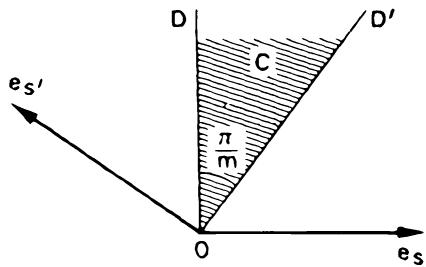
\includegraphics[keepaspectratio]{images/part001_dfbe6528.jpg}}\\
图 2

\subsection{W 在诸室的并中的基本域}

我们沿用第 4 号的记号。对于 \(s \in S\) ，用 \(H_s\) 表示 \(E^*\) 中正交于 \(e_s\) 的超平面，用 \(\overline{A_s}\) 表示由 \(x^* \in E^*\) （满足 \(\langle x^*, e_s \rangle \geqslant 0\) ）构成的集合，并用 \(\overline{C}\) 表示诸 \(\overline{A_s}\) （\(s \in S\) ）的交。对于弱拓扑 \(\sigma(E^*, E)\) （它由 \(E^*\) 与 \(E\) 之间的对偶性定义；《拓扑向量空间》，第 II 章，§6，第 2 号），诸 \(\overline{A_s}\) 是闭半空间，而 \(\overline{C}\) 是一个闭凸锥。此外，\(\overline{C}\) 是 C 的闭包；事实上，若 \(x^* \in \overline{C}\) 且 \(y^* \in C\) ，则 \(x^* + ty^* \in C\) （对每个实数 \(t > 0\) ），且 \(x^* = \lim_{t \to 0} (x^* + ty^*)\) 。

对于 \(X\subset S\) ，置

\[
C _ {X} = \left(\bigcap_ {s \in X} H _ {s}\right) \cap \left(\bigcap_ {s \in S - X} A _ {s}\right).
\]

我们有 \(C_X \subset \overline{C}\) ，\(C_{\varnothing} = C\) 且 \(C_S = \{0\}\) 。诸集合 \(C_X\) （\(X \in B(S)\) ）构成 \(\overline{C}\) 的一个划分。

另一方面，回忆（第 IV 章，§1，第 8 号）\(\mathbf{W}_{\mathbf{X}}\) 表示 \(\mathbf{W}\) 的由 \(\mathbf{X}\) 生成的子群。显然 \(w(x^{*}) = x^{*}\) （对于 \(w \in \mathbf{W}_{\mathbf{X}}\) 与 \(x^{*} \in \mathbf{C}_{\mathbf{X}}\) ）。

命题 5. 设 \(X, X' \subset S\) 且 \(w, w' \in W\) 。若 \(w(C_X) \cap w'(C_{X'}) \neq \emptyset\) ，则 \(X = X'\) ，\(wW_X = w'W_{X'}\) 且 \(w(C_X) = w'(C_{X'})\) 。

我们立即化归到 \(w' = 1\) 的情形。证明对长度 \(n\) （\(w\) 的长度）作归纳。若 \(n = 0\) ，断言是显然的。若 \(l(w) > 0\) ，则存在 \(s \in S\) 使 \(l(sw) = l(w) - 1\) ，于是（参见~第 4 号末尾）\(w(C) \subset s(A_s)\) ，从而 \(w(\overline{C}) \subset s(\overline{A_s})\) 。由于 \(\overline{C} \subset \overline{A_s}\) ，由此得到

\[
\overline {{{\mathrm{C}}}} \cap w (\overline {{{\mathrm{C}}}}) \subset \mathrm{H} _ {s}.
\]

于是 \(s(x^{*}) = x^{*}\) （对所有 \(x^{*} \in \overline{\mathrm{C}} \cap w(\overline{\mathrm{C}})\) ），从而更对所有

\[
x ^ {*} \in \mathrm{C} _ {\mathrm{X} ^ {\prime}} \cap w (\mathrm{C} _ {\mathrm{X}}).
\]

因此，关系 \(C_{X'} \cap w(C_X) \neq \varnothing\) 一方面蕴含 \(C_{X'} \cap H_s \neq \varnothing\) ，从而 \(s \in X'\) ；另一方面蕴含 \(C_{X'} \cap sw(C_X) \neq \varnothing\) 。于是归纳假设表明 \(X = X'\) 且 \(swW_X = W_{X'} = W_X\) ，故 \(sw \in W_X\) ，且 \(w \in W_X\) （由于 \(s \in W_X\) ）。由此得到 \(wW_X = W_{X'}\) 以及 \(w(C_X) = C_X = C_{X'}\) 。

推论. 设 X 是 S 的子集，\(x^{*}\) 是 \(C_{X}\) 的一个元素。\(x^{*}\) 在 W 中的稳定子是 \(W_{X}\) 。

现在设 U 为诸 \(w(\overline{\mathbf{C}})\) （\(w \in W\) ）的并，并设 F 为 U 中形如 \(w(\mathrm{C}_{X})\) 的子集（其中 \(X \subset S\) 且 \(w \in W\) ）所成的集合。由上所述，F 是 U 的一个划分。

命题 6. (i) 锥 U 是凸的。

\begin{enumerate}
\def\labelenumi{(\roman{enumi})}
\setcounter{enumi}{1}
\item
  U 中所含的每个闭线段只与 \(\mathfrak{F}\) 中的有限多个元素相交。
\item
  锥 \(\overline{\mathbf{C}}\) 是 W 在 U 上作用的一个基本域。
\end{enumerate}

为证明 (iii)，只需证明：若 \(x^{*}, y^{*} \in \overline{\mathbb{C}}\) 与 \(w \in \mathbb{W}\) 满足 \(w(x^{*}) = y^{*}\) ，则 \(x^{*} = y^{*}\) 。现在存在两个子集 \(\mathbf{X}\) 与 \(\mathbf{Y}\) （\(\mathbf{S}\) 中的），使得 \(x^{*} \in \mathrm{C}_{\mathbf{X}}\) 且 \(y^{*} \in \mathrm{C}_{\mathbf{Y}}\) ；我们有 \(w(\mathrm{C}_{\mathbf{X}}) \cap \mathrm{C}_{\mathbf{Y}} \neq \emptyset\) ，而命题 5 表明 \(\mathbf{X} = \mathbf{Y}\) 且 \(w \in \mathrm{W}_{\mathbf{X}}\) ，这就蕴含 \(x^{*} = y^{*}\) 。

现在设 \(x^{*}, y^{*} \in \mathrm{U}\) ；我们将证明线段 \([x^{*}y^{*}]\) 被 \(\mathfrak{F}\) 中有限多个元素所覆盖，这就同时建立了 (i) 与 (ii)。把 \(x^{*}\) 与 \(y^{*}\) 用 \(\mathrm{W}\) 的同一个元素来变换，我们可以假设 \(x^{*} \in \overline{\mathrm{C}}\) 。设 \(w \in \mathrm{W}\) 满足 \(y^{*} \in w(\overline{\mathrm{C}})\) 。我们对 \(w\) 的长度作归纳论证。对于 \(s \in \mathrm{S}\) ，关系 \(w(\overline{\mathrm{C}}) \not\subset \overline{\mathrm{A}_{s}}\) 等价于 \(w(\mathrm{C}) \notin \mathrm{A}_{s}\) ，从而等价于 \(l(sw) < l(w)\) （参见~第 4 号）。于是第 IV 章 §1 第 8 号的命题 7 表明，只存在有限多个 \(s \in \mathrm{S}\) 满足 \(w(\overline{\mathrm{C}}) \not\subset \overline{\mathrm{A}_{s}}\) 。于是，集合 \(T\) （由那些 \(s \in S\) 组成，其中 \(\langle y^{*}, e_{s} \rangle < 0\) ）是有限的。另一方面，交 \(\overline{\mathrm{C}} \cap [x^{*}y^{*}]\) 是一个闭线段 \([x^{*}z^{*}]\) 。若 \(z^{*} = y^{*}\) ，即若 \(y^{*} \in \overline{\mathrm{C}}\) ，则存在子集 \(X\) 与 \(Y\) （\(S\) 中的），使得 \(x^{*} \in C_{X}\) 且 \(y^{*} \in C_{Y}\) 。开线段 \(|x^{*}y^{*}|\) 于是含于 \(C_{X \cap Y}\) ，故 \([x^{*}y^{*}] \subset C_{X} \cup C_{Y} \cup C_{X \cap Y}\) 。若 \(z^{*} \neq y^{*}\) ，则存在 \(s \in T\) 使 \(z^{*} \in H_{s}\) 。于是 \(w(C) \not\subset A_{s}\) 且 \(l(sw) < l(w)\) 。从而归纳假设表明，线段 \([z^{*}y^{*}] = s([z^{*}(s(y^{*}))])\) 被 \(\mathfrak{F}\) 的有限多个元素所覆盖，因而

\[
\left[ x ^ {*} y ^ {*} \right] = \left[ x ^ {*} z ^ {*} \right] \cup \left[ z ^ {*} y ^ {*} \right]
\]

因为 \([x^{*}z^{*}]\subset \overline{\mathbf{C}}.\)

\subsection{Coxeter 群的几何表示的不可约性}

我们沿用前面各号的记号，并假设 S 有限。

命题 7. 假设 (W,S) 是不可约的（第 IV 章，§1，第 9 号）。设 \(\mathbf{E}^0\) 是 E 的关于 \(\mathbf{B}_{\mathbf{M}}\) 与 E 正交的子空间。群 W 平凡地作用于 \(\mathbf{E}^0\) ，并且 E 的每个异于 E 且在 W 下稳定的子空间都含于 \(\mathbf{E}^0\) 。

若 \(x \in \mathrm{E}^0\) ，则 \(\sigma_s(x) = x - 2\mathrm{B}_{\mathrm{M}}(e_s, x)e_s = x\) 对所有 \(s \in \mathrm{S}\) 成立。由于 \(\mathrm{W}\) 由 \(\mathrm{S}\) 生成，由此可知 \(\mathrm{W}\) 平凡地作用于 \(\mathrm{E}^0\) 。

设 \(E'\) 是 \(E\) 的一个在 \(W\) 下稳定的子空间。设 \(s, s' \in S\) 是在图 \(\Gamma\) （即 \((W, S)\) 的图；第 IV 章，§1，第 9 号）中相连的两个元素；回忆这意味着 \(m(s, s') \geqslant 3\) 。假设 \(e_s \in E'\) 。则 \(\sigma_{s'}(e_s) \in E'\) ，且由于 \(e_{s'}\) 在 \(\sigma_{s'}(e_s)\) 中的系数非零，我们有 \(e_{s'} \in E'\) 。由于 \(\Gamma\) 连通，由此可知，若 \(E'\) 含有某个 \(e_s\) ，则它含有它们全体并与 \(E\) 重合。除这一情形外，由 §2 第 2 号命题 3 可知，对所有 \(s \in S\) ，\(E'\) 含于超平面 \(H_s\) （正交于 \(e_s\) ）。由于诸 \(H_s\) 的交等于 \(E^0\) ，命题得证。

推论. 假设 (W, S) 是不可约的。则：

\begin{enumerate}
\def\labelenumi{\alph{enumi})}
\item
  若 \(\mathrm{B_M}\) 非退化，则 W-模 E 是绝对单的。
\item
  若 \(\mathrm{B_M}\) 退化，则 W-模 E 不是半单的。
\end{enumerate}

在情形 \(a\) ，命题 7 表明 \(E\) 是单的，从而也是绝对单的（§ 2，第 1 号，命题 1）。

在情形 \(b\) ，有 \(\mathrm{E}^0 \neq 0\) ，\(\mathrm{E} \neq \mathrm{E}^0\) （因为 \(\mathrm{B}_{\mathrm{M}} \neq 0\) ），且命题 7 表明 \(\mathrm{E}^0\) 没有在 W 下稳定的补空间；因此 W-模 E 不是半单的。

\subsection{有限性判别准则}

我们沿用前面各号的记号，并假设 S 有限。

定理 2. 以下性质等价：

\begin{enumerate}
\def\labelenumi{(\arabic{enumi})}
\item
  W 是有限的。
\item
  型 \(B_{M}\) 是正的且非退化的。
\item
  \(\Longrightarrow\) (2). 设 \(S = \bigcup_{i} S_{i}\) 是 \(S\) 分解为连通分支的分解（第 IV 章，§ 1，第 9 号），并设 \(W = \prod_{i} W_{i}\) 是 \(W\) 的相应分解。空间 \(E\) 可与诸空间 \(E_{i} = R^{S_{i}}\) 的直和等同，而 \(B_{M}\) 可与诸相应的型 \(B_{M_{i}}\) 的直和等同。于是我们化归到 \((W, S)\) 不可约的情形。由于假设 \(W\) 有限，\(E\) 是半单的 \(W\) -模（附录，命题 2）。由命题 5 的推论可知 \(E\) 是绝对单的。设 \(B'\) 是 \(E\) 上一个正的非退化型，并设 \(B''\) 是它在 \(W\) 下诸变换的和。由于 \(B''\) 在 \(W\) 下不变，它与 \(B_{M}\) 成比例（ \(\S 2\) ，第 1 号，命题 1）；由于 \(B_{M}(e_{s}, e_{s}) = 1\) （对所有 \(s \in S\) ）成立，比例系数 \(>0\) ，而由于 \(B''\) 是正的，\(B_{M}\) 亦然，这就证明了 (2)。
\item
  \(\Longrightarrow\) (1). 若 \(B_{M}\) 正且非退化，则正交群 \(\mathbf{O}(B_{M})\) 是紧的（《积分》第 VII 章，§3，第 1 号）。由于 \(\sigma(W)\) 是 \(\mathbf{O}(B_{M})\) 的离散子群（定理 1 的推论 3），可知 \(\sigma(W)\) 有限，从而 W 亦有限。证毕。
\end{enumerate}

下面的结果已在证明过程中得到建立：

推论. 若 \((\mathrm{W},\mathrm{S})\) 不可约且有限，则 \(\mathbf{E}\) 是绝对单的 W-模。

定理 2 所提供的有限性判别准则使得可以对所有有限 Coxeter 群进行分类（参见~第 VI 章，§4）。我们在这里只限于下面的初步结果：

命题 8. 若 W 有限，则 (W, S) 的图是一个森林（第 IV 章，附录）。

若不然，这个图将包含一个回路 \((s_{1},\ldots,s_{n})\) ，其中 \(n\geqslant3\) 。置 \(m_{i}=m(s_{1},s_{i+1})\) （\(1\leqslant i<n\) ）及 \(m_{n}=m(s_{n},s_{1})\) ，这就意味着对所有 i 有 \(m_{i}\geqslant3\) 。设

\[
x = e _ {s _ {1}} + \dots + e _ {s _ {n}}.
\]

于是 \(\mathrm{B_M}(x,x) = n + 2\sum_{i < j}\mathrm{B_M}(e_{s_i},e_{s_j})\) 。而

\[
\mathrm{B} _ {\mathrm{M}} (e _ {s _ {i}}, e _ {s _ {i + 1}}) = - \cos \frac {\pi}{m _ {i}} \leqslant - \cos \frac {\pi}{3} \leqslant - \frac {1}{2},
\]

对 \(\mathrm{B}_{\mathbb{M}}(e_{s_n}, e_{s_i})\) 同样如此。由于和中其余各项 \(\leqslant 0\) ，我们得到

\[
\mathrm{B} _ {\mathrm{M}} (x, x) \leqslant n - n = 0,
\]

这与 \(B_{M}\) 正且非退化相矛盾。

推论. 若 (W, S) 不可约且有限，则其图是一棵树。

事实上，连通的森林是树。

与 §3 结果的比较。

首先设 \((W,S)\) 是一个有限 Coxeter 群。用 \((x|y)\) 表示型 \(\mathrm{B}_{\mathbf{M}}(x,y)\) ；由定理 2，这是 E 上的一个标量积。对所有 \(s \in S\) ，设 \(H_{s}\) 是与正交反射 \(\sigma_{s}\) 相伴随的超平面，并设 \(\mathfrak{H}\) 为超平面族 \(w(\mathrm{H}_{s})\) （其中 \(s \in S\) ，\(w \in W\) ）。设 \(C_{0}\) 为由 \(x \in E\) （满足 \((x|e_{s}) > 0\) ，对所有 \(s \in S\) ）所成的集合。最后，借助 \(\sigma\) 把 W 与空间 E 的正交群 \(\mathbf{O}(\mathbf{E})\) 的一个子群等同起来。

命题 9. 按照前面的记号，W 是 O(E) 的由关于 \(\mathfrak{H}\) 中诸超平面的反射所生成的子群。它是一个本质的群（§3，第 7 号），且 C0 是 E 相对于 \(\mathfrak{H}\) 的一个室。

第一个断言是平凡的。另一方面，若 \(x \in E\) 在 W 下不变，则它与所有 \(e_{s}\) 正交，从而为零；这表明 W 是本质的。最后，同构 \(E \to E^{*}\) （由 \(B_{M}\) 定义）把 \(C_{0}\) 变为第 4 号中的集合 C；在那里证明的性质 \((P_{n})\) 表明，对所有 \(w \in W\) 与所有 \(s \in S\) ，\(w(C_0)\) 不与 \(H_s\) 相交。由此可知 \(C_0\) 含于 \(\mathfrak{H}\) 中诸超平面之并的补集 U，而由于 \(C_0\) 在 U 中连通、开且闭，它是 E 相对于 \(\mathfrak{H}\) 的一个室。证毕。

我们可以把 §3 中证明的所有性质应用于 W 与 \(C_{0}\) 。特别地，\(\overline{C_{0}}\) 是 W 在 E 上作用的一个基本域（换句话说，第 6 号中定义的锥 U 等于整个 E）。

反之，设 E 是一个有限维实向量空间，配备标量积 \((x|y)\) ，并设 W 是 E 的一个本质的有限位移群且保持 0 固定；假设 W 由反射生成。设 \(C_{0}\) 是 E 相对于 W 的一个室（参见~§3），并设 S 是相对于 \(C_{0}\) 的墙的正交反射所成的集合。则 (W, S) 是一个有限 Coxeter 系统（§3，第 2 号，定理 1）。此外，若 \(s \in S\) ，用 \(H_{s}\) 表示 \(C_{0}\) 的与 s 相应的墙，并用 \(e_{s}\) 表示正交于 \(H_{s}\) 且关于 \(H_{s}\) 与 \(C_{0}\) 位于同侧的单位向量。若 \((m(s, s'))\) 表示 (W, S) 的 Coxeter 矩阵，则 §3 的命题 3 与 7 表明

\[
(e _ {s} | e _ {s ^ {\prime}}) = - \cos (\pi / m (s, s ^ {\prime}))
\]

并且诸 \(e_{s}\) 构成 E 的一个基。于是 W 在 E 上的自然表示可与第 3 号的表示 \(\sigma\) 等同。

\subsection{\texorpdfstring{\(\mathbf{B}_{\mathrm{M}}\) 为正且退化的情形}{B\_M 为正且退化的情形}}

在本号中，我们假设 S 有限，\((W, S)\) 不可约，且型 \(B_{M}\) 是正的且退化的。

引理 2. 正交补 \(\mathbf{E}^0\) —— 即 \(\mathbf{E}\) 关于 \(\mathbf{B}_{\mathbf{M}}\) 的正交补 —— 是 1 维的；它由一个元素 \(v = \sum_{s\in S}v_s e_s\) （其中 \(v_{s} > 0\) 对所有 \(s\) 成立）生成。

这由 §3 第 5 号的引理 4（应用于以 \(\mathrm{B}_{\mathbb{M}}(e_s, e_{s'})\) 为元素的矩阵）得出。

设 \(v = \sum_{s} v_s e_s\) 是满足引理 2 的条件且使 \(\sum_{s} v_s = 1\) 的向量，并设 A 是 \(E^*\) 中由 \(y^* \in E^*\) （满足 \(\langle v, y^* \rangle = 1\) ）构成的仿射超平面。若 T 表示 \(v\) 在 \(E^*\) 中的正交补，则 A 具有一个仿射空间的自然结构，以 T 为平移空间。此外，型 \(B_M\) 通过过渡到商在 \(E/E^0\) 上定义一个非退化标量积，从而也在其对偶 T 上定义；这给出仿射空间 A 上的一个欧氏结构（《代数》第 IX 章，§6，第 6 号）。

设 G 是 \(\mathbf{GL}(\mathbf{E})\) 的由保持 v 与 \(B_{M}\) 不变的自同构构成的子群；若 \(g \in G\) ，则逆步映射 \({}^{t}g^{-1}\) 保持 A 与 T 稳定，且通过限制到 A 上定义 A 的一个位移 \(i(g)\) （参见~§3）。立即可见这给出从 G 到 A 的位移群的一个同构。此外，A 的点 a 的稳定子 \(G_{a}\) 可与 Hilbert 空间 T 的正交群等同，从而是紧的。另一方面，G 是一个在无穷远处可数的局部紧群，而 A 是一个 Baire 空间：由此（《积分》第 VII 章，附录，引理 2）可知映射 \(\psi : g \mapsto g(a)\) 定义从 \(G/G_a\) 到 A 的一个同胚。于是 G 适当地作用于 A（《一般拓扑》第 III 章，§4，第 2 号，命题 5）。由于 W 是 G 的子群，它可与 A 的一个位移群等同。我们将证明这个群满足 §3 的假设。更确切地说：

命题 10. 赋予离散拓扑的群 W 适当地作用于 A；它由正交反射生成；它是无限的、不可约的且本质的（§3，第 7 号）。交 C ∩ A 是 W 在 A 中的一个室。若 L\_s 表示 A 中由 A 与 E* 的正交于 e\_s 的超平面相交而得的超平面，则诸 L\_s （对于 s ∈ S）是 C ∩ A 的墙。若 ε\_s 是 T 中正交于 L\_s 且与 C ∩ A 位于 L\_s 同侧的单位向量，则 (ε\_s\textbar ε\_t) = -cos(π/m(s,t)) （对于 s,t ∈ S），且 W 的 Coxeter 矩阵（§3，第 4 号）与 M 等同。

由定理 1 的推论 3，W 在 \(\mathbf{GL}(\mathbf{E})\) 中离散，从而在 \(\mathbf{G}\) 中离散，且适当地作用于 A。设 \(s \in S\) 。由于 \(\operatorname{Card} S \geqslant 2\) ，\(\mathbf{E}^*\) 中正交于 \(e_s\) 的超平面不正交于 \(v\) ，它与 A 的交 \(\mathbf{L}_s\) 确是超平面。于是与 \(s\) 相应的位移是保持 \(\mathbf{L}_s\) 的所有点固定的 2 阶位移：它必然是与 \(\mathbf{L}_s\) 相伴随的正交反射。由此可知 W 由正交反射生成。定理 2 现在表明它是无限的，而命题 7 表明它是本质的且不可约的。

由于 C 是一个开单形锥，其墙是方程为 \(\langle x^{*}, e_{s} \rangle = 0\) （对于 \(s \in S\) ）的超平面，交 \(C \cap A\) 是 A 中诸 \(L_{s}\) 之并的补集的一个凸的、从而连通的开且闭子集。此外，\(C \cap A\) 非空，因为若 \(x^{*} \in C\) ，我们有 \(\langle x^{*}, v \rangle = \sum_{s} v_{s} \langle x^{*}, e_{s} \rangle > 0\) 且 \(\langle x^{*}, v \rangle^{-1} x^{*} \in C \cap A\) 。由此可知 \(C \cap A\) 是 A 相对于诸 \(L_{s}\) 的系统的一个室。此外，\(w(C \cap A) \cap L_{s} = \varnothing\) （对所有 \(w \in W\) ；参见~第 4 号，性质 \((\mathrm{P}_{n})\) ）成立，因而 \(C \cap A\) 是 A 相对于由诸 \(L_{s}\) 经 W 的元素变换所得的系统的一个室；由 §3 第 2 号定理 1 的推论可知，\(C \cap A\) 是 A 相对于 W 的一个室。

设 \(a_{s}^{*}\) 是单形 \(C \cap A\) 的不在 \(L_{s}\) 中的顶点。我们有

\[
\left\langle a _ {s} ^ {*}, e _ {t} \right\rangle = 0
\]

对 \(s,t\in \mathrm{S}\) 且 \(s\neq t\) 成立，且

\[
\langle a _ {s} ^ {*}, e _ {s} \rangle = v _ {s} ^ {- 1} \langle a _ {s} ^ {*}, v \rangle = v _ {s} ^ {- 1}.
\]

设 \(\varepsilon_{s}\) 是 T 中由下列关系式定义的向量：

\[
\left(\varepsilon_ {s} \mid a _ {s} ^ {*} - a _ {t} ^ {*}\right) = v _ {s} ^ {- 1} \text {for} t \in S, t \neq s.
\]

向量 \(\varepsilon_{s}\) 正交于 \(L_{s}\) ，且关于超平面 \(L_{s}\) 与 \(C \cap A\) 位于同侧。此外

\[
\left(\varepsilon_ {s} \mid a _ {s} ^ {*} - a _ {t} ^ {*}\right) = \left\langle e _ {s}, a _ {s} ^ {*} - a _ {t} ^ {*} \right\rangle \text {for all} s, t \in S
\]

这表明 \(\varepsilon_{s}\) 是 \(e_{s}\) 的类在从 \(E/E^{0}\) 到 T 的同构（由二次型 \(B_{M}\) 给出）下的像。由此得到

\[
(\varepsilon_ {s} | \varepsilon_ {t}) = \mathrm{B} _ {\mathrm{M}} (e _ {s}, e _ {t}).
\]

因此 \(\varepsilon_{s}\) 是单位向量，而命题 10 的最后一个断言得证。

配备群 W 的欧氏仿射空间 A 称为与 Coxeter 矩阵 M 相伴随的空间，我们记之为 \(A_{M}\) 。

命题 10 有一个逆命题：

命题 11. 设 W 是欧氏仿射空间 A 的一个位移群，满足 §3 的假设。假设 W 是无限的、本质的且不可约的。则与 W 的 Coxeter 矩阵 M 相伴随的型 \(B_{M}\) 是正的且退化的，并且存在唯一的从与 M 相伴随的仿射空间 \(A_{M}\) 到 A 的同构，它与 W 的作用交换。这个同构把 \(A_{M}\) 的标量积变为 A 的标量积的倍数。

设 \(C_0\) 是 A 的一个室，并设 S 是相对于 \(C_0\) 的墙的正交反射所成的集合。若 \(\eta_s\) 表示正交于与反射 s 相伴随的超平面 \(N_s\) 且关于 \(N_s\) 与 \(C_0\) 位于同侧的单位向量（§3，命题 3），则型 \(B_M\) 满足 \(B_M(e_s, e_t) = (\eta_s | \eta_t)\) （对于 \(s, t \in S\) ）。从而它是正的。由于诸 \(\eta_s\) 线性相关（§3，第 9 号，命题 8），它是退化的。

于是我们可以把前面的构造应用于 M。沿用与上面相同的记号，\((\varepsilon_{s}|\varepsilon_{t}) = (\eta_{s}|\eta_{t})\) ，且存在唯一的 Hilbert 空间同构 \(\varphi\) ，从 T 到 A 的平移空间，使得 \(\varphi(\varepsilon_{s}) = \eta_{s}\) 。设 a 与 b 是 \(C_{0}\) 的两个不同顶点，\(s_{0}\) 是 S 中使 \(a \notin N_{s_{0}}\) 的反射。置 \(\lambda = (\eta_{s}|a - b)\) ，并设 \(\psi\) 是由下式定义的从 \(A_{M}\) 到 A 的仿射双射

\[
\psi \left(a _ {s _ {0}} + x\right) = a + v _ {s _ {0}} \lambda \varphi (x) \text {for} x \in \mathrm{T}.
\]

于是立即可见 \(\psi(\mathrm{L}_{s}) = \mathrm{N}_{s}\) （对所有 \(s \in S\) ），且 \(\psi\) 把 \(A_{M}\) 的标量积变为 A 上标量积的倍数。立即得到 \(\psi\) 与 W 的作用交换。最后，\(\psi\) 的唯一性是明显的，因为例如 \(a_{s}\) 是 \(A_{M}\) 中在诸反射 \(t \in S, t \neq s\) 下不变的唯一点。

\section{对称代数中的不变量}

\subsection{分次代数的 Poincaré 级数}

设 K 是一个有单位元且不退化为 0 的交换环。设 M 是一个 Z 型分次 K-模，\(M_{n}\) 是 M 中次数为 n 的齐次元素所成的集合。假设每个 \(M_{n}\) 都是自由的且有限型的。于是秩 \(\operatorname{rk}_{\mathbf{K}}(\mathbf{M}_{n})\) 对所有 n 有定义（《交换代数》第 II 章，§5，第 3 号）。

定义 1. 若存在 \(n_0 \in \mathbf{Z}\) 使 \(M_n = 0\) （对于 \(n \leqslant n_0\) ），则形式级数 \(\sum_{n \geqslant n_0} \mathrm{rk}_K(M_n) T^n\) （\(\mathbf{Q}((T))\) 的一个元素）称为 \(M\) 的 Poincaré 级数，记为 \(P_M(T)\) 。

设 \(M'\) 是另一个 Z 型分次 K-模，\((M_n')_{n \in \mathbf{Z}}\) 是它的分次。假设 \(M_n'\) 对小于某个数的 n 为零。则

\[
\mathrm{P} _ {\mathrm{M} \oplus \mathrm{M} ^ {\prime}} (\mathrm{T}) = \mathrm{P} _ {\mathrm{M}} (\mathrm{T}) + \mathrm{P} _ {\mathrm{M} ^ {\prime}} (\mathrm{T})\tag{1}
\]

而若给 \(\mathbf{M} \otimes_{\mathbf{K}} \mathbf{M}'\) 赋予总分次（《代数》第 II 章，§11，第 5 号），则

\[
\mathrm{P} _ {\mathrm{M} \otimes \mathrm{M} ^ {\prime}} (\mathrm{T}) = \mathrm{P} _ {\mathrm{M}} (\mathrm{T}) \mathrm{P} _ {\mathrm{M} ^ {\prime}} (\mathrm{T}).\tag{2}
\]

命题 1. 设 \(S = \bigoplus_{n \geqslant 0} S_n\) 是一个交换分次 K-代数，具有一个由齐次且代数无关的元素组成的生成元组 \((x_1, x_2, \ldots, x_m)\) 。设 \(d_i\) 是 \(x_i\) 的次数，并假设 \(d_i > 0\) （对所有 \(i\) ）。则诸 \(S_n\) 在 \(K\) 上是自由的且有限秩的，并且

\[
\mathrm{P} _ {\mathrm{S}} (\mathrm{T}) = \prod_ {i = 1} ^ {m} (1 - \mathrm{T} ^ {d _ {i}}) ^ {- 1}.\tag{3}
\]

事实上，S 可与张量积 \(K[x_{1}] \otimes \cdots \otimes K[x_{m}]\) 等同，后者赋予总分次。\(K[x_{i}]\) 的 Poincaré 级数是

\[
\sum_ {n \geqslant 0} \mathrm{T} ^ {n d _ {i}} = (1 - \mathrm{T} ^ {d _ {i}}) ^ {- 1},
\]

于是只需应用 (2)。

在命题 1 的假设下，我们将称 S 是 K 上的一个分次多项式代数。

推论. 诸次数 \(d_{i}\) 由 S 确定，至多相差次序。

事实上，\(\mathrm{P}_{\mathrm{S}}(\mathrm{T})\) 的逆是多项式 \(\mathrm{N}(\mathrm{T}) = \prod_{i=1}(1 - \mathrm{T}^{d_i})\) ，从而是唯一确定的。若 q 是一个整数 \(\geqslant 1\) 且 \(\zeta \in C\) 是一个本原 q 次单位根，则根 \(\zeta\) 在 \(\mathrm{N}(\mathrm{T})\) 中的重数等于 \(d_{i}\) 中是 q 的倍数的个数。当 q 充分大时这个数为零。于是等于 q 的 \(d_{i}\) 的个数由递降归纳唯一确定。

诸整数 \(d_{i}\) 称为 S 的特征次数。当 K 是域时，它们的个数等于 S 在 K 上的超越次数；在一般情形我们也把它称为 S 在 K 上的超越次数。它是多项式 N(T) 的根 1 的重数。

设 \(S = \bigoplus_{n \geqslant 0} S_n\) 是一个交换分次 K-代数，\(R = \bigoplus_{n \geqslant 0} R_n\) 是 S 的一个分次子代数。假设每个 \(R_n\) 都是自由的且有限型的，且 R-模 S 具有一个由齐次元素 \(z_1, z_2, \ldots, z_N\) （次数分别为 \(f_1, f_2, \ldots, f_N\) ）组成的有限基。于是，若用 M 表示分次 K-模 \(\sum_{j=1}^{N} Kz_j\) ，则分次 K-模 S 同构于 \(R \otimes_K M\) ，从而每个 \(S_n\) 都是自由的且有限型的，并且

\[
P _ {S} (T) = P _ {M} (T) P _ {R} (T) = \left(\sum_ {j = 1} ^ {N} T ^ {f _ {j}}\right) P _ {R} (T).\tag{4}
\]

命题 2. 沿用前面的记号，并假设 \(S\) 与 \(R\) 是分次多项式代数。

\begin{enumerate}
\def\labelenumi{(\roman{enumi})}
\item
  R 与 S 有相同的超越次数 \(r\) （在 \(K\) 上）。
\item
  设 \(p_1, \ldots, p_r\) （分别为 \(q_1, \ldots, q_r\) ）是 \(S\) （分别为 \(R\) ）的特征次数。则
\end{enumerate}

\[
\prod_ {i = 1} ^ {r} \left(1 - \mathrm{T} ^ {q _ {i}}\right) = \left(\sum_ {j = 1} ^ {\mathrm{N}} \mathrm{T} ^ {f _ {j}}\right) \prod_ {i = 1} ^ {r} \left(1 - \mathrm{T} ^ {p _ {i}}\right).
\]

\begin{enumerate}
\def\labelenumi{(\roman{enumi})}
\setcounter{enumi}{2}
\tightlist
\item
  \(Np_{1}p_{2}\ldots p_{r}=q_{1}q_{2}\ldots q_{r}.\)
\end{enumerate}

公式 (4) 首先表明根 1 的重数在多项式 \(\mathrm{P}_{\mathrm{S}}(\mathrm{T})^{-1}\) 与 \(\mathrm{P}_{\mathrm{R}}(\mathrm{T})^{-1}\) 中相同，再考虑到 (3)，就同时证明了 (i) 与 (ii)。

由 (ii) 得到

\[
\prod_ {i = 1} ^ {r} \left(1 + \mathrm{T} + \mathrm{T} ^ {2} + \dots + \mathrm{T} ^ {q _ {i} - 1}\right) = \left(\sum_ {j = 1} ^ {\mathrm{N}} \mathrm{T} ^ {f _ {j}}\right) \prod_ {i = 1} ^ {r} \left(1 + \mathrm{T} + \mathrm{T} ^ {2} + \dots + \mathrm{T} ^ {p _ {i} - 1}\right).
\]

在此关系中置 \(\mathrm{T} = 1\) 即得 (iii)。

注. 设 \(S = K[X_1, \ldots, X_n]\) 是 \(K\) 上的一个分次多项式代数，\(d_i\) 是 \(X_i\) 的次数，\(F(X_1, \ldots, X_n)\) 是一个次数为 \(m\) 的 \(S\) 的齐次元素。则

\[
\sum_ {i = 1} ^ {n} d _ {i} X _ {i} \frac {\partial F}{\partial X _ {i}} = m F.\tag{5}
\]

事实上，立即可见把每个次数为 p 的齐次元素 z 变为 pz 的、从 S 到 S 的 K-线性映射 D 是 S 的一个求导。于是

\[
m \mathrm{F} (\mathrm{X} _ {1}, \dots , \mathrm{X} _ {n}) = \mathrm{D} (\mathrm{F} (\mathrm{X} _ {1}, \dots , \mathrm{X} _ {n})) = \sum_ {i = 1} ^ {n} \mathrm{D} (\mathrm{X} _ {i}) \frac {\partial \mathrm{F}}{\partial \mathrm{X} _ {i}} = \sum_ {i = 1} ^ {n} d _ {i} \mathrm{X} _ {i} \frac {\partial \mathrm{F}}{\partial \mathrm{X} _ {i}}.
\]

\subsection{有限线性群的不变量：模性质}

设 K 是一个交换环，V 是一个 K-模，G 是一个作用于 V 的群。我们知道 V 的每个自同构唯一地开拓为对称代数 \(S = \mathbf{S}(V)\) 的自同构，从而 G 作用于这个代数。若 \(x \in S\) 且 \(g \in G\) ，用 \(g_{S}.x\) 表示 x 在 g 下的像。设 R 是 S 中由在 G 下不变的元素构成的子代数 \(S^{G}\) 。

假设 G 有限，V 有限型，且 K 是 noether 的。于是 S 是一个有限型 R-模，而 R 是一个有限型 K-代数（《交换代数》第 V 章，§1，第 9 号，定理 2）。假设 S 是整的，并设 N 是它的分式域。R 的分式域 L 是 N 中在 G 下不变的元素所成的集合（出处同前，命题 23 的推论），故 N 是 L 的一个 Galois 扩张。N 的每个元素都可写成 z/t，其中 \(z \in S\) 且 \(t \in R\) （出处同前，命题 23）。由《代数》第 II 章 §7 第 10 号命题 26 的推论 3，R-模 S 的秩是 {[}N : L{]}。假设 G 忠实地作用于 V。于是 N 在 L 上的 Galois 群可与 G 等同，故 {[}N : L{]} = Card G；从而

\[
\operatorname{rk} _ {\mathsf {R}} (\mathrm{S}) = [ \mathrm{N}: \mathrm{L} ] = \operatorname{Card} (\mathrm{G}).\tag{6}
\]

对任意分次代数 \(A = A_{0} \oplus A_{1} \oplus \cdots \oplus A_{n} \oplus \cdots\) ，用 \(A_{+}\) 表示理想 \(\bigoplus_{n > 0} A_{n}\) 。

定理 1. 设 K 是一个交换域，V 是 K 上一个有限维向量空间，S = S(V) 是 V 的对称代数，G 是 V 的一个有限自同构群，R 是 S 中由在 G 下不变的元素组成的分次子代数。假设 G 由伪反射生成（§2，第 1 号），且 q = Card(G) 与 K 的特征互素。则 R-模 S 具有一个由 q 个齐次元素组成的基。

\begin{enumerate}
\def\labelenumi{\alph{enumi})}
\item
  由于 \(S/(R_{+}S)\) 的每个子模在 \(R_0 = K\) 上都是自由的，只需（《代数》第 II 章，§11，第 4 号，命题 7）证明从 \(R_{+} \otimes_{R} S\) 到 \(S\) 的典范同态是单射。对任意 R-模 \(E\) ，用 \(T(E)\) 表示 R-模 \(\text{Ker}(R_{+} \otimes_{R} E \to E)\) （*换句话说，\(T(E) = \text{Tor}_{1}^{R}(R/R_{+}, E)_*\) ）。若 \(E, E'\) 是两个 R-模而 \(u\) 是从 \(E\) 到 \(E'\) 的同态，则同态 \(1 \otimes u\) （从 \(R_{+} \otimes E\) 到 \(R_{+} \otimes E'\) ）通过限制到 \(T(E)\) 上定义一个从 \(T(E)\) 到 \(T(E')\) 的同态，我们记之为 \(T(u)\) 。若 \(u'\) 是从 \(E'\) 到某个 R-模 \(E''\) 的同态，则有 \(T(u' \circ u) = T(u') \circ T(u)\) 。于是，若 G R-线性地作用于 \(E\) ，则 G 作用于 \(T(E)\) 。
\item
  群 G R-线性地作用于 S，从而也作用于 T(S)。此外，T(S) 具有一个分次 S-模的自然结构。我们首先证明，若 \(g \in G\) ，则 g 把 T(S) 的每个元素 x 变为模 \(S_{1}T(S)\) 与 x 同余的元素。只需对 g 是伪反射的情形证明这一点。此时存在 V 中一个非零向量 v，使得 \(g(x) - x \in Kv\) （对所有 \(x \in V\) ）。由于 V 生成 S，由此可知 \(g_{S}\) 平凡地作用于 S/Sv。于是，对任意 \(y \in S\) ，存在 S 中一个元素 \(h(y)\) 使得
\end{enumerate}

\[
g _ {\mathrm{S}} (y) - y = h (y) v.
\]

由于 S 是整的且 v 非零，这个元素由 y 唯一确定；立即可见 h 是 R-模 S 的一个次数为 -1 的自同态。于是 \(g_{S} - 1_{S} = m_{v} \circ h\) ，其中 \(m_{v}\) 表示 S 中比率为 v 的位似。由此，

\[
\mathrm{T} (g _ {\mathrm{S}}) - 1 _ {\mathrm{T(S)}} = \mathrm{T} (g _ {\mathrm{S}} - 1 _ {\mathrm{S}}) = \mathrm{T} (m _ {v}) \circ \mathrm{T} (h),
\]

其像含于 \(vT(S)\) ，这就证明了我们的断言。

\begin{enumerate}
\def\labelenumi{\alph{enumi})}
\setcounter{enumi}{2}
\tightlist
\item
  我们证明 \(T(S)\) 中在 G 下不变的任何元素为零。事实上，设 Q 是 R-模 S 的由下式定义的自同态
\end{enumerate}

\[
\mathrm{Q} (y) = q ^ {- 1} \sum_ {g \in G} g _ {\mathrm{S}} (y)
\]

（对所有 \(y \in S\) ）。则 \(Q(S) = R\) 。于是我们可以写 \(Q = i \circ Q'\) ，其中 \(Q'\) 是从 R-模 S 到 R-模 R 的同态，而 i 表示 R 到 S 中的典范单射。从而 \(T(Q) = T(i) \circ T(Q')\) ，且 \(T(Q') = 0\) ，因为 \(T(R) = \text{Ker}(R_{+} \otimes R \to R) = 0\) 。于是

\[
0 = \mathrm{T} (\mathrm{Q}) = q ^ {- 1} \sum_ {g \in \mathrm{G}} \mathrm{T} (g _ {\mathrm{S}}).
\]

而 \(q^{-1} \sum_{g \in G} T(g_S)\) 保持 \(T(S)\) 中在 G 下不变的元素不动。因此这些元素为零。

\begin{enumerate}
\def\labelenumi{\alph{enumi})}
\setcounter{enumi}{3}
\tightlist
\item
  假设 \(T(S) \neq 0\) 。在 \(T(S)\) 中存在一个次数最小的非零齐次元素 \(u \neq 0\) 。由 b)，u 在 G 下不变。由 c)，u = 0。这是矛盾，故 \(T(S) = 0\) 。证毕。
\end{enumerate}

注. 1) 由《代数》第 II 章 §11 第 4 号命题 7 可知，若 \((z_{1},\ldots ,z_{q})\) 是 S 的一个齐次元素族，其典范像在 \(\mathrm{S / (R_+S)}\) 中构成 \(\mathrm{S / (R_+S)}\) 在 K 上的基，则 \((z_{1},\ldots ,z_{q})\) 是 S 在 R 上的基。

\begin{enumerate}
\def\labelenumi{\arabic{enumi})}
\setcounter{enumi}{1}
\tightlist
\item
  设 \(g\) 是 \(V\) 的一个伪反射，其阶 \(n \geqslant 2\) 有限且与 \(K\) 的特征互素。由 Maschke 定理（附录，命题 2），\(V\) 可分解为 \(D \oplus H\) ，其中 \(H\) 是由 \(V\) 中在 \(g\) 下不变的元素组成的超平面，而 \(D\) 是一条直线，\(g\) 在其上通过乘以一个本原 \(n\) 次单位根作用。当 \(K = R\) 时，这仅当 \(n = 2\) 时才可能，此时 \(g\) 是一个反射；在这种情形，定理 1 所适用的群是有限 Coxeter 群。（相反，对 K = C，定理 1 适用于某些不是 Coxeter 群的群。）\(^{3}\)
\end{enumerate}

定理 2. 沿用定理 1 的假设与记号。

\begin{enumerate}
\def\labelenumi{(\roman{enumi})}
\item
  存在 \(S\) 的一个分次向量子空间，它构成 \(R_{+}S\) 在 \(S\) 中的补，且在 \(G\) 下稳定。
\item
  设 U 是这样一个补。从 \(U \otimes_{K} R\) 到 S 的典范同态是 G-模的同构，且 G 在 U（分别为 S）中的表示同构于 G 在 K（分别为 R）上的正则表示。
\end{enumerate}

事实上，对任意整数 \(n \geqslant 0\) ，K-向量空间 \(S_n\) 与 \((R_+S) \cap S_n\) 在 \(G\) 下稳定，且由 Maschke 定理（附录，命题 2）可知存在一个 G-稳定的子空间 \(U_n\) ，它构成 \((R_+S) \cap S_n\) 在 \(S_n\) 中的补。于是 \(\sum_{n \geqslant 0} U_n\) 是 \(R_+S\) 在 \(S\) 中的一个 G-稳定的补，由此得 (i)。

设 U 是 S 的一个分次向量子空间，它在 S 中构成 \(R_{+}S\) 的补且在 G 下稳定。由注 1，K-向量空间 U 的每个基也是 R-模 S 的基，从而是 S 的分式域 N 在 R 的分式域 L 上的基。于是 L-向量空间 N 可与 \(U \otimes_{K} L\) 等同。由于 U 在 G 下稳定，这一等同与 G 的作用相容。G 在 L 上的群代数 \(L[G]\) 可与代数 \(K[G] \otimes_{K} L\) 等同。L 的 Galois 扩张 N 具有正规基（《代数》第 V 章，§10，第 9 号，定理 6），这可以解释为：N（视为 \(L[G]\) -模）同构于 G 在 L 上的正则表示的模。由于 U 在 K 上有限维，由附录命题 1 可知 \(K[G]\) -模 U 同构于 G 在 K 上的正则表示。我们的断言由此立得。

\subsection{有限线性群的不变量：环论性质}

定理 3. 我们沿用定理 1 的假设与记号。在 \(R_{+}\) （R 的理想）的由齐次元素组成的生成元组的集合中，取一个极小元 \((\alpha_{1},\ldots,\alpha_{l})\) 。设 \(k_{i}\) 是 \(\alpha_{i}\) 的次数。假设诸 \(k_{i}\) 与 K 的特征指数互素。则 \(l=\dim V\) ，诸 \(\alpha_{i}\) 生成 K-代数 R，且在 K 上代数无关。特别地，R 是 K 上超越次数为 l 的一个分次多项式 K-代数。

关于 \(k_{i}\) 所作的假设是多余的，但对有限 Coxeter 群的应用而言无关紧要，因为那时 K = R。参见第 5 号，我们将在那里给出定理 3 的另一个证明。

定理 3 由命题 2 (i)、定理 1 以及下面的引理得出：

引理 1. 设 K 是一个交换域，S 是一个分次多项式 K-代数，R 是 S 的一个有限型分次子代数，使得 R-模 S 具有一个由齐次元素组成的基 \((z_{\lambda})_{\lambda \in \Lambda}\) 。在 \(R_{+}\) （R 的理想）的由齐次元素组成的生成元组的集合中，取一个极小元 \((\alpha_{1}, \ldots, \alpha_{s})\) 。假设对所有 i，次数 \(k_{i}\) （\(\alpha_{i}\) 的）与 K 的特征指数 p 互素。则诸 \(\alpha_{i}\) 生成 K-代数 R 且在 K 上代数无关。

由《代数》第 II 章 § 11 第 4 号命题 7，关于 \(\alpha_{i}\) 所作的假设等价于说它们是齐次的，且它们的像在 K-向量空间 \(R_{+}/(R_{+})^{2}\) 中构成该空间的基。这一条件在基域扩张下不变；于是我们可以化归到基域为完满的情形。

族 \((\alpha_{1},\ldots,\alpha_{s})\) 生成代数 R（《交换代数》第 III 章，§1，第 2 号，命题 1）。我们用反证法，假设这个族在 K 上不是代数无关的。

\begin{enumerate}
\def\labelenumi{\arabic{enumi})}
\tightlist
\item
  我们首先证明存在诸族
\end{enumerate}

\[
\left(\beta_ {i}\right) _ {1 \leqslant i \leqslant s}, \quad \left(y _ {k}\right) _ {1 \leqslant k \leqslant r}, \quad \left(d _ {i k}\right) _ {1 \leqslant i \leqslant s, 1 \leqslant k \leqslant r}
\]

它们由 S 的齐次元素组成，且满足下列性质：

\[
\beta_ {i} \in R \text {for all} i, \text {and the} \beta_ {i} \text {are not all zero};\tag{7}
\]

\[
\deg y _ {k} > 0 \text {   for   all   } k;\tag{8}
\]

\[
\alpha_ {i} = \sum_ {k = 1} ^ {r} d _ {i k} y _ {k} \quad \text { for   all } i;\tag{9}
\]

\[
\sum_ {i = 1} ^ {s} \beta_ {i} d _ {i k} = 0 \quad \text { for   all } k.\tag{10}
\]

设 \(X_{1},\ldots,X_{s}\) 是未定元，并给 \(K[X_{1},\ldots,X_{s}]\) 赋予使 \(X_{i}\) 的次数为 \(k_{i}\) 的分次代数结构。存在非零齐次元素 \(H(X_{1},\ldots,X_{s})\) ，它属于 \(K[X_{1},\ldots,X_{s}]\) ，使得 \(H(\alpha_{1},\ldots,\alpha_{s})=0\) ；取 H 为次数最小的。若 \(\partial H/\partial X_{i}\neq0\) ，则多项式 \(\frac{\partial H}{\partial X_{i}}(\alpha_{1},\ldots,\alpha_{s})\) 是 R 的一个非零齐次元素；若 \(p\neq1\) ，则 H 不具有 \(H_{1}^{p}\) （其中 \(H_{1}\in K[X_{1},\ldots,X_{s}]\) ）的形式。取

\[
\beta_ {i} = k _ {i} \frac {\partial \mathrm{H}}{\partial \mathrm{X} _ {i}} (\alpha_ {1}, \dots , \alpha_ {s}).
\]

由于 K 是完满的，多项式 \(\partial H/\partial X_{i} \in K[X_{1},\ldots,X_{s}]\) 不全为零（《代数》第 V 章，§1，第 3 号，命题 4）；鉴于关于 \(k_{i}\) 的假设，诸 \(\beta_{i}\) 亦不全为零。

另一方面，S 可与一个分次多项式代数 \(K[x_{1},\ldots,x_{r}]\) 等同，其中 \(x_{1},\ldots,x_{r}\) 是适当的未定元，次数为适当的 \(m_{i}>0\) 。设 \(D_{k}\) 是 S 上关于 \(x_{k}\) 的偏导数。取 \(d_{ik} = k_i^{-1}\mathrm{D}_k(\alpha_i)\) 。则等式 (10) 成立，因为其左边是 \(\mathrm{D}_k(\mathrm{H}(\alpha_1,\dots ,\alpha_s))\) 。另一方面，若置 \(y_{1} = m_{1}x_{1},\ldots ,y_{r} = m_{r}x_{r}\) ，则等式 (9) 由第 1 号的等式 (5) 得出。

\begin{enumerate}
\def\labelenumi{\arabic{enumi})}
\setcounter{enumi}{1}
\tightlist
\item
  设 \(\mathfrak{b}\) 是 \(R\) 的由诸 \(\beta_{i}\) 生成的理想；存在下述集合的一个子集 \(J\) ：
\end{enumerate}

\[
\mathrm{I} = \{1, 2, \dots , s \}
\]

使得 \((\beta_{i})_{i\in\mathbb{J}}\) 是 b 的一个极小生成元组。则 \(J\neq\varnothing\) ，因为 \(b\neq0\) 。我们将由 (9) 与 (10) 推出：若 \(i\in J\) ，则 \(\alpha_{i}\) 是诸 \(\alpha_{j}\) （\(j\neq i\) ）的 R-线性组合，这与 \((\alpha_{1},\ldots,\alpha_{s})\) 的极小性矛盾，从而完成证明。

存在 R 的齐次元素 \(\gamma_{ji}\) ( \(i \in \mathrm{J}, j \in \mathrm{I} - \mathrm{J}\) ) 使得

\[
\beta_ {j} = \sum_ {i \in J} \gamma_ {j i} \beta_ {i} (j \in I - J).\tag{11}
\]

考虑到 (11)，公式 (10) 给出

\[
\sum_ {i \in \mathrm{J}} \beta_ {i} \left(d _ {i k} + \sum_ {j \in \mathrm{I} - \mathrm{J}} \gamma_ {j i} d _ {j k}\right) = 0.\tag{12}
\]

置

\[
u _ {i k} = d _ {i k} + \sum_ {j \in I - J} \gamma_ {j i} d _ {j k}.\tag{13}
\]

于是

\[
\sum_ {i \in J} \beta_ {i} u _ {i k} = 0.\tag{14}
\]

写 \(u_{ik} = \sum_{\lambda \in \Lambda} \delta_{ik\lambda} z_\lambda\) ，其中诸 \(\delta_{ik\lambda}\) 属于 R。关系式 (14) 蕴含 \(\sum_{i \in J} \beta_i \delta_{ik\lambda} = 0\) （对所有 \(k\) 与 \(\lambda\) ）。若某个 \(\delta_{ik\lambda}\) 有一个次数为 0 的非零齐次分量，则前面的等式将蕴含某个 \(\beta_i\) ( \(i \in J\) ) 是其余元素的 R-线性组合，与 \((\beta_i)_{i \in J}\) 的极小性矛盾。于是 \(\delta_{ik\lambda} \in R_+\) ，从而 \(u_{ik} \in R_+ S\) （对所有 \(i\) 与 \(k\) ）。于是存在 \(u_{ikh} \in S\) 使得 \(u_{ik} = \sum_{h=1}^{s} u_{ikh} \alpha_h\) ，换句话说，由 (13)，

\[
d _ {i k} + \sum_ {j \in I - J} \gamma_ {j i} d _ {j k} = \sum_ {h = 1} ^ {s} u _ {i k h} \alpha_ {h}.\tag{$(15)_{ik}$}
\]

把 \((15)_{ik}\) 的两边乘以 \(y_{k}\) ，并对固定的 i ∈ J 与 \(k = 1, 2, \ldots, r\) 相加；鉴于 (9)，我们得到

\[
\alpha_ {i} + \sum_ {j \in I - J} \gamma_ {j i} \alpha_ {j} = \sum_ {h = 1} ^ {s} \sum_ {k = 1} ^ {r} u _ {i k h} y _ {k} \alpha_ {h}.
\]

取两边的次数为 \(k_i\) 的齐次分量。由于 \(\deg y_k > 0\) ，\(\alpha_i\) 是诸 \(\alpha_j\) （\(j \neq i\) ）的 S-线性组合。由于 S 在 R 上自由且 \(\alpha_1, \ldots, \alpha_s \in \mathrm{R}\) ，由此可知 \(\alpha_i\) 是诸 \(\alpha_j\) （\(j \neq i\) ）的 R-线性组合（《交换代数》第 I 章，§3，第 5 号，命题 9 d))。

推论. 在定理 3 的假设与记号下，R 的特征次数之积是 Card(G)。

事实上，\(\operatorname{rk}_{\mathrm{R}}(S) = \operatorname{Card}(G)\) （公式 (6)，第 2 号）。S 的特征次数都等于 1。于是推论由第 1 号命题 2 (iii) 得出。

引理 2. 设 K 是一个交换域，V 是 K 上一个有限维向量空间，\(S = \bigoplus_{n \geqslant 0} S_n\) 是 V 的对称代数，s 是 V 的一个自同态，\(s^{(n)}\) 是 s 到 \(S_n\) 的典范开拓。则当 T 表示一个未定元时，我们在 K{[}{[}T{]}{]} 中有

\[
\sum_ {n = 0} ^ {\infty} \operatorname{Tr} (s ^ {(n)}) \mathrm{T} ^ {n} = (\det (1 - s \mathrm{T})) ^ {- 1}.
\]

必要时扩张基域，我们可以假设 K 是代数闭的。设 \((e_{1},\ldots,e_{r})\) 是 V 的一个基，s 关于它的矩阵是下三角的，并设 \(\lambda_{1},\ldots,\lambda_{r}\) 是这个矩阵的对角元素。关于按字典序排列的基 \((e_{1}^{i(1)}\ldots e_{r}^{i(r)})_{i(1)+\cdots+i(r)=n}\) （\(S_{n}\) 的），\(s^{(n)}\) 的矩阵是下三角的，其对角元素是诸乘积 \(\lambda_{1}^{i(1)}\ldots\lambda_{r}^{i(r)}\) 。于是

\[
\operatorname{Tr} \left(s ^ {(n)}\right) = \sum_ {i (1) + \dots + i (r) = n} \lambda_ {1} ^ {i (1)} \dots \lambda_ {r} ^ {i (r)},
\]

从而

\[
\begin{array}{l} \sum_ {n = 0} ^ {\infty} \operatorname{Tr} (s ^ {(n)}) \mathrm{T} ^ {n} = \left(\sum_ {n = 0} ^ {\infty} \lambda_ {1} ^ {n} \mathrm{T} ^ {n}\right) \left(\sum_ {n = 0} ^ {\infty} \lambda_ {2} ^ {n} \mathrm{T} ^ {n}\right) \ldots \left(\sum_ {n = 0} ^ {\infty} \lambda_ {r} ^ {n} \mathrm{T} ^ {n}\right) \\ \qquad = (1 - \lambda_ {1} \mathrm{T}) ^ {- 1} (1 - \lambda_ {2} \mathrm{T}) ^ {- 1} \ldots (1 - \lambda_ {r} \mathrm{T}) ^ {- 1} \\ \qquad = (\det (1 - s \mathrm{T})) ^ {- 1}. \end{array}
\]

引理 3. 设 K、V 与 S 如引理 2 中所述，G 是 V 的一个有限自同构群，q 是 G 的阶，R 是 S 中由在 G 下不变的元素组成的分次子代数。假设 K 的特征为 0。则 R 的 Poincaré 级数是

\[
q ^ {- 1} \sum_ {g \in G} (\det (1 - g T)) ^ {- 1}.
\]

事实上，自同态 \(f = q^{-1} \sum_{g \in G} g^{(n)}\) 是 \(S_n\) 到 \(R_n\) 上的一个投影，故 \(\operatorname{Tr}(f) = \dim_K S_n^G\) 。于是 \(R\) 的 Poincaré 级数是

\[
q ^ {- 1} \sum_ {g \in G} \left(\sum_ {n = 0} ^ {\infty} (\operatorname{Tr} g ^ {(n)}) T ^ {n}\right),
\]

于是只需应用引理 2。

命题 3. 在定理 3 的假设与记号下，设 H 是属于 G 且异于 1 的伪反射所成的集合。假设 K 的特征为 0。则 \(\operatorname{Card}(\mathrm{H}) = \sum_{i=1}^{l}(k_i - 1)\) 。

由附录命题 3，我们可以假设 K 是代数闭的。对任意 \(g \in G\) ，设 \(\lambda_{1}(g), \ldots, \lambda_{l}(g)\) 是它的特征值。由于每个 \(g \in G\) 都可对角化（附录，命题 2），g = 1 当且仅当所有 \(\lambda_{i}(g)\) 都等于 1，而 \(g \in H\) 当且仅当等于 1 的 \(\lambda_{i}(g)\) 的个数是 l - 1（此时我们用 \(\lambda(g)\) 表示异于 1 的特征值）。第 1 号的命题 1 与引理 3 证明

\[
q \prod_ {i = 1} ^ {l} (1 - T ^ {k _ {i}}) ^ {- 1} = \sum_ {g \in G} (\det (1 - g T)) ^ {- 1}\tag{16}
\]

在 \(\mathbf{K}[[\mathbf{T}]]\) 中成立，从而在 \(\mathbf{K}(\mathbf{T})\) 中成立。于是，我们在 \(\mathbf{K}(\mathbf{T})\) 中有

\[
q \frac {(1 - T) ^ {l - 1}}{\prod_ {i = 1} ^ {l} (1 - T ^ {k _ {i}})} = \frac {1}{1 - T} + \sum_ {g \in H} \frac {1}{1 - \lambda (g) T} + \sum_ {g \neq 1, g \notin H} \frac {(1 - T) ^ {l - 1}}{\det (1 - g T)},
\]

它可以写成

\[
\begin{array}{c} \frac {q - \prod_ {i = 1} ^ {l} (1 + T + \cdots + T ^ {k _ {i} - 1})}{(1 - T) \prod_ {i = 1} ^ {l} (1 + T + \cdots + T ^ {k _ {i} - 1})} \\ = \sum_ {g \in H} \frac {1}{1 - \lambda (g) T} + \sum_ {g \neq 1, g \notin H} \frac {(1 - T) ^ {l - 1}}{\det (1 - g T)}. \end{array}\tag{17}
\]

由此可知 \(q - \prod_{i=1}^{l} (1 + T + \cdots + T^{k_i - 1})\) 在 T = 1 处为零，故 \(q = k_1 k_2 \ldots k_l\) ，这一点我们已由定理 3 的推论得知。鉴此，设 \(Q(T)\) 是多项式 \((1 - T)^{-1}(q - \prod_{i=1}^{l} (1 + T + \cdots + T^{k_i - 1}))\) 。对等式 \((1 - T)Q(T) = q - \prod_{i=1}^{l} (1 + T + \cdots + T^{k_i - 1})\) 求导并置 T = 1，我们看到 \(-Q(1)\) 是下式在 T = 1 处的值

\[
\begin{array}{l} - \frac {d}{d t} \left(\prod_ {i = 1} ^ {l} (1 + T + \dots + T ^ {k _ {i} - 1})\right) \\ = - \sum_ {i = 1} ^ {l} \left((1 + 2 T + \dots + (k _ {i} - 1) T ^ {k _ {i} - 2}) \prod_ {j \neq i} (1 + T + \dots + T ^ {k _ {j} - 1})\right) \end{array}
\]

于是

\[
Q (1) = \sum_ {i = 1} ^ {l} \frac {\left(k _ {i} - 1\right) k _ {i}}{2} \prod_ {j \neq i} k _ {j} = \left(\prod_ {j = 1} ^ {l} k _ {j}\right) \left(\sum_ {i = 1} ^ {l} \frac {k _ {i} - 1}{2}\right).
\]

回到 (17)，我们另一方面有

\[
Q (1) = \left(\prod_ {j = 1} ^ {l} k _ {j}\right) \left(\sum_ {g \in H} \frac {1}{1 - \lambda (g)}\right).
\]

于是，

\[
\sum_ {i = 1} ^ {l} \frac {k _ {i} - 1}{2} = \sum_ {g \in H} \frac {1}{1 - \lambda (g)}.\tag{18}
\]

现在，\(\mathbf{G}\) 中保持一个给定超平面的点固定的元素保持该超平面的补直线稳定（附录，命题 2），从而由《代数》第 V 章 §11 第 1 号定理 1 构成一个循环子群 \(\mathbf{G}'\) （\(\mathbf{G}\) 的）。设 \(t\) 是 \(\mathbf{G}'\) 的阶；\(\lambda(g)\) （\(g \in \mathbf{G}'\) ）的值是 \(\theta, \theta^2, \ldots, \theta^{t-1}\) ，其中 \(\theta\) 是一个本原 \(t\) 次单位根。我们有 \(\frac{1}{1-\theta^i} + \frac{1}{1-\theta^{t-i}} = 1\) ，故 \(\sum_{g \in \mathbf{G}', g \neq 1} \frac{1}{1-\lambda(g)} = \frac{1}{2}(t-1) = \frac{1}{2}\mathrm{Card}(\mathrm{H} \cap \mathrm{G}')\) 。于是等式 (18) 证明了命题。

注. 当 \(\mathbf{K} = \mathbf{R}\) 、\(\mathbf{G}\) 是一个 Coxeter 群且 \(\mathbf{H}\) 是属于 \(\mathbf{G}\) 的反射所成的集合时，我们知道（§ 3）\(\mathbf{H}\) 的元素与 \(\mathbf{V}\) 的墙一一对应。

命题 4. 在定理 3 的假设与记号下，假设 K 的特征 \(\neq 2\) 。则 \(-1 \in G\) 当且仅当 R 的特征次数 \(k_{1}, \ldots, k_{l}\) 都是偶数。

设 \(f\) 是代数 \(S\) 的自同构，它开拓 \(-1\) （\(V\) 的自同构）。则 \(f(z) = (-1)^{\deg z}z\) （对所有齐次 \(z\) ，\(S\) 中的）。于是，若 \(-1 \in G\) ，则 \(R\) 的每个奇次数的齐次元素为零，且诸 \(k_i\) 都是偶数。反之，若诸 \(k_i\) 都是偶数，则 \(R\) 的每个元素在 \(f\) 下不变，且 Galois 理论表明 \(-1 \in G\) 。

\subsection{反不变元素}

我们沿用定理 3 的假设与记号，并假设 K 的特征为 0。称 S 的一个元素 z 是 G 下反不变的，如果

\[
g (z) = (\det g) ^ {- 1} z
\]

对所有 \(g\in G\) 成立

设 H 是属于 G 且异于 1 的伪反射所成的集合。对所有 \(g \in H\) ，存在 \(e_{g} \in V\) 与 \(f_{g} \in V^{*}\) 使得

\[
g (x) = x + f _ {g} (x) e _ {g} \quad \text {   for   all   } x \in V.
\]

命题 5. (i) 设 \(\mathrm{D}\) 是 \(\prod_{g \in \mathrm{H}} e_g\) （\(\mathrm{S}\) 的一个元素）。\(\mathrm{S}\) 中在 \(\mathrm{G}\) 下反不变的元素是 \(\mathrm{RD}\) 的元素。

\begin{enumerate}
\def\labelenumi{(\roman{enumi})}
\setcounter{enumi}{1}
\tightlist
\item
  把 S 与多项式代数 \(\mathrm{K}[\mathrm{X}_1,\dots ,\mathrm{X}_l]\) 等同（通过选取 V 的一个基 \((\mathrm{X}_1,\dots ,\mathrm{X}_l)\) ），并设 \((\mathrm{P}_1,\dots ,\mathrm{P}_l)\) 是 S 中生成代数 R 的代数无关齐次元素（定理 3）。则 Jacobi 行列式 \(\mathrm{J} = \det \left(\frac{\partial\mathrm{P}_t}{\partial\mathrm{X}_j}\right)\) 具有 \(\lambda D\) 的形式，其中 \(\lambda \in K^*\) 。
\end{enumerate}

\begin{enumerate}
\def\labelenumi{\alph{enumi})}
\tightlist
\item
  按照 (ii) 中的记号，我们有
\end{enumerate}

\[
d \mathrm{P} _ {1} \wedge d \mathrm{P} _ {2} \wedge \dots \wedge d \mathrm{P} _ {l} = \mathrm{J} d \mathrm{X} _ {1} \wedge d \mathrm{X} _ {2} \wedge \dots \wedge d \mathrm{X} _ {l},
\]

于是，对所有 \(g \in G\) ，

\[
\begin{array}{c} g (\mathrm{J}) (\det g)   d \mathrm{X} _ {1} \wedge \ldots \wedge d \mathrm{X} _ {l} = g (\mathrm{J})   d (g \mathrm{X} _ {1}) \wedge \ldots \wedge d (g \mathrm{X} _ {l}) \\ = g (d \mathrm{P} _ {1} \wedge \ldots \wedge d \mathrm{P} _ {l}) = d \mathrm{P} _ {1} \wedge \ldots \wedge d \mathrm{P} _ {l} = \mathrm{J}   d \mathrm{X} _ {1} \wedge \ldots \wedge d \mathrm{X} _ {l}, \end{array}
\]

从而 J 在 G 下反不变。另一方面，S 的分式域 N 是 R 的分式域 E 的一个 Galois 扩张（第 2 号）；若 \(\Delta\) 是 E 的一个取值于 N 的扩域 \(\Omega\) 中的求导，则 \(\Delta\) 开拓为 N 的一个取值于 \(\Omega\) 中的求导（《代数》第 V 章，§ 16，第 4 号，定理 3）；由于诸 \(P_{i}\) 代数无关，由此可知 \(dP_{1} \wedge \ldots \wedge dP_{l} \neq 0\) ，从而 \(J \neq 0\) 。

\begin{enumerate}
\def\labelenumi{\alph{enumi})}
\setcounter{enumi}{1}
\item
  设 \(z\) 是 \(S\) 的一个在 \(G\) 下反不变的元素。我们证明 \(z\) 被 \(D\) 整除（在 \(S\) 中）。设 \(a\) 是 \(V\) 中一个非零向量。\(G\) 中保持 \(Ka\) 稳定的元素保持一个补超平面 \(L\) 稳定（附录，命题 2）；\(G\) 的一个保持 \(Ka\) 稳定的元素是 1 或以 \(a\) 为向量的伪反射，当且仅当它在 \(L\) 上诱导 1；于是以 \(a\) 为向量且属于 \(G\) 的伪反射与 1 一起构成一个循环子群 \(G'\) （\(G\) 的）；设 \(t\) 是它的阶。存在一个基 \((X_1, \ldots, X_l)\) （\(V\) 的），使得 \(a = X_1\) ，\(X_2 \in L, \ldots, X_l \in L\) ，且 \(z\) 可与一个多项式 \(P(X_1, \ldots, X_l)\) （系数在 \(K\) 中）等同。由 \(g(z) = (\det g)^{-1}z\) （对 \(g \in G'\) ），我们看到 \(X_1\) 在 \(P(X_1, \ldots, X_l)\) 中只以模 \(t\) 同余于 -1 的指数出现。于是 \(P(X_1, \ldots, X_l)\) 被 \(X_1^{t-1} = a^{t-1}\) 整除。而现在 \(D\) 是诸 \(a^{t-1}\) （对这些 \(a \in V\) ，\(t > 1\) ）的乘积（至多差一个标量因子），且 \(S\) 的这些元素两两互素。由于 \(S\) 是唯一分解的，\(z\) 被 \(D\) 整除。
\item
  由 a) 与 b)，J 在 S 中被 D 整除。而现在
\end{enumerate}

\[
\deg \mathrm{J} = \sum_ {i = 1} ^ {l} (k _ {i} - 1) = \operatorname{Card} (\mathrm{H})
\]

（命题 3），故 \(\deg J = \deg D\) ，从而 \(J = \lambda D\) ，其中 \(\lambda \in K\) 。由于 \(J \neq 0\) ，\(\lambda \in K^*\) 。这就证明了 (ii)。

\begin{enumerate}
\def\labelenumi{\alph{enumi})}
\setcounter{enumi}{3}
\tightlist
\item
  证明的 a) 与 c) 部分表明 D 在 G 下反不变。其次，若 \(y \in R\) ，则显然 yD 在 G 下反不变。最后，若 \(z \in S\) 在 G 下反不变，我们在 b) 中已见存在 \(y \in S\) 使 z = yD。由于 S 是整的，\(y \in R\) 。这就证明了 (i)。
\end{enumerate}
